\documentclass[czech]{beamer}
\usepackage[utf8]{inputenc}
\usepackage[T1]{fontenc}
\usepackage[czech]{babel}
\usepackage{amsmath}

\usetheme{Madrid}
\usecolortheme{default}

\title[Raytracing]{Raytracing: když přesnost je zbytečný luxus}
\author{David Nápravník}
\date{24.09.2025}
\institute[MFF]{Matematicko-fyzikální fakulta UK}

\begin{document}
\titlegraphic{%
  \vspace*{\fill}
  \fontsize{4}{4.8}\normalfont
  \hfill Pokud není uvedeno jinak\\ \hfill obrázky David Nápravník\\ \hfill CC BY 4.0
}
\maketitle


\begin{frame}{Co je ray tracing}
\begin{itemize}
  \item Sledování pohybu fotonů napříč scénou
  \item Podloženo fyzikálními zákony
  \item Dříve jen ve filmu, ale dnes i v reálném čase
\end{itemize}
\vfill
\centering 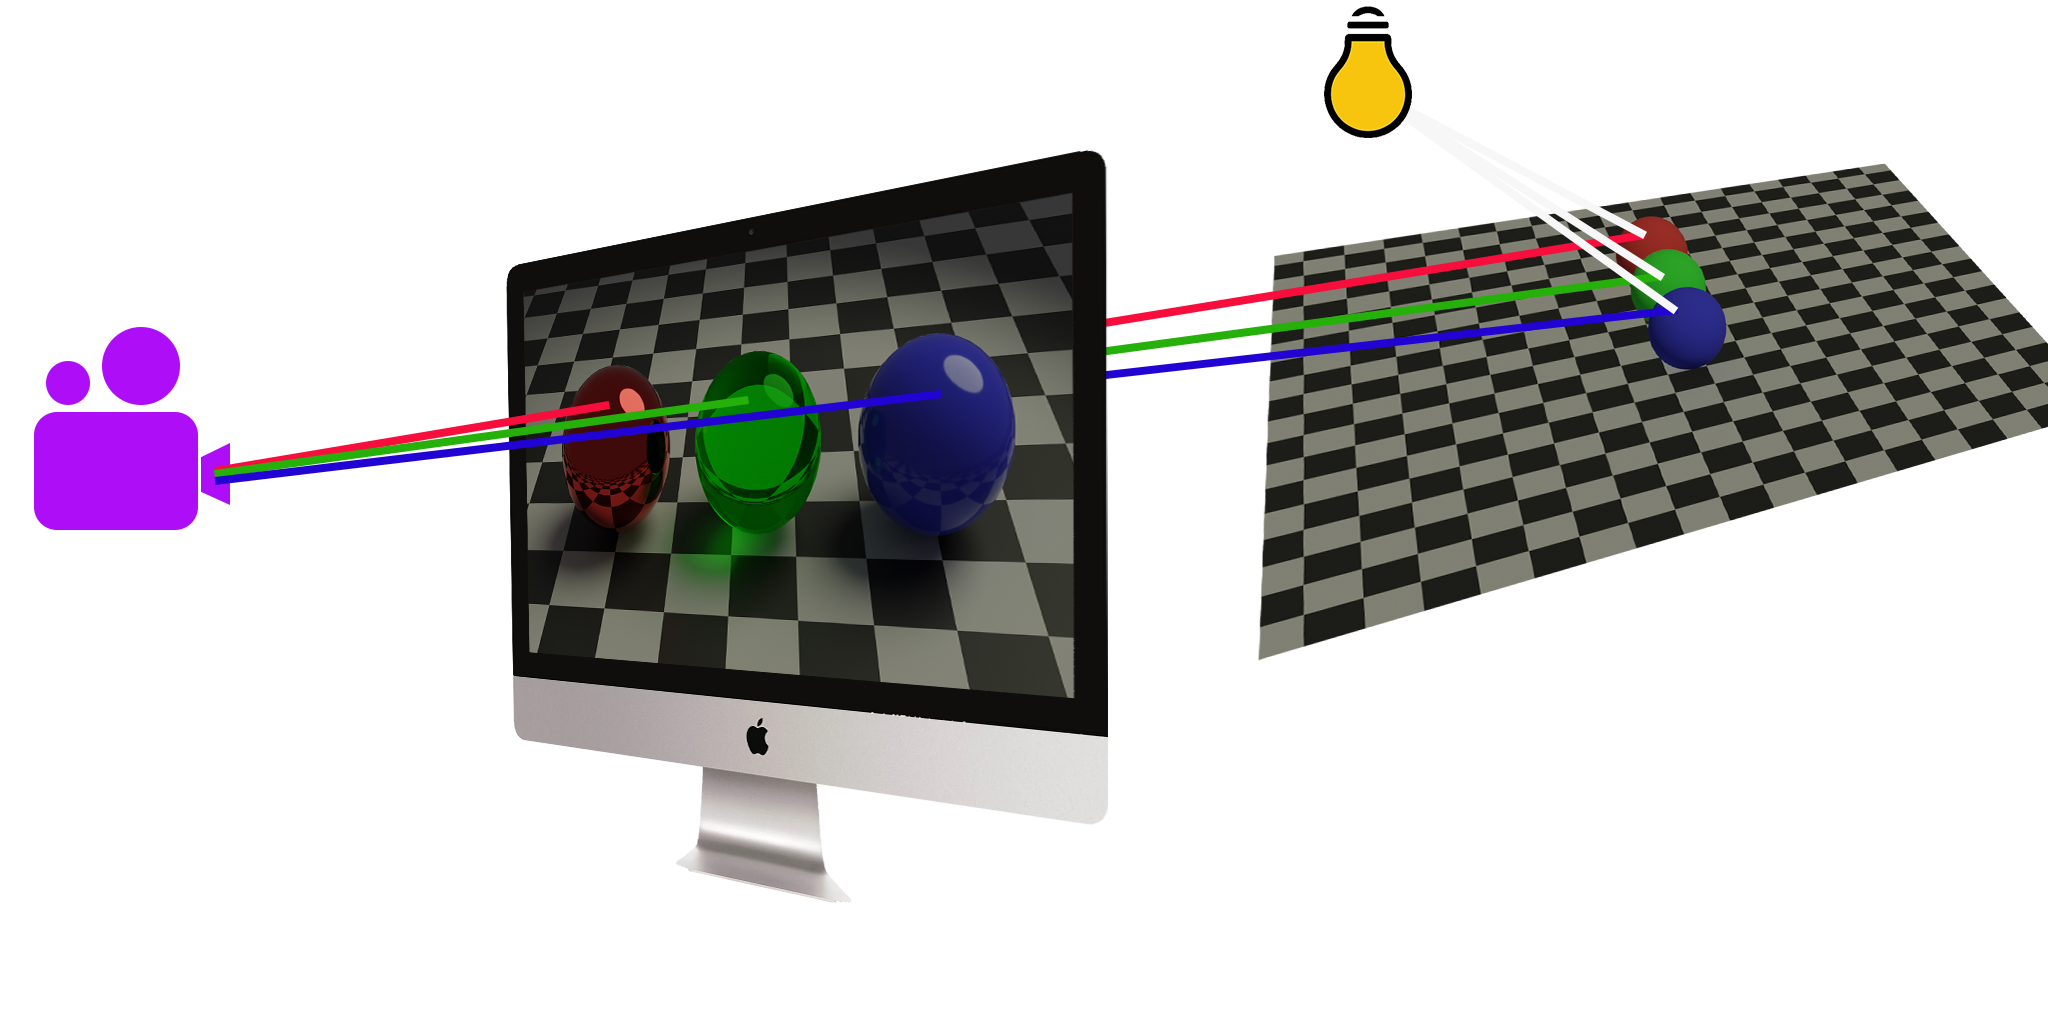
\includegraphics[width=0.9\textwidth]{img/raytracing composite.png}
\end{frame}


\begin{frame}{Renderovací rovnice}
\begin{itemize}
  \item Matematické vyjádření pohybu světla ve scéně
  \item Výstupem je osvětlení specifického bodu ve scéně
\end{itemize}

\begin{block}{Renderovací rovnice (Kajiya 1986)}
\[
L_o(\omega_o) = L_e(\omega_o) + \int_{\Omega} f_r(\omega_i \rightarrow \omega_o)\, L_i(\omega_i)\, \cos \theta_i\, d\omega_i\
\]
\end{block}
\centering 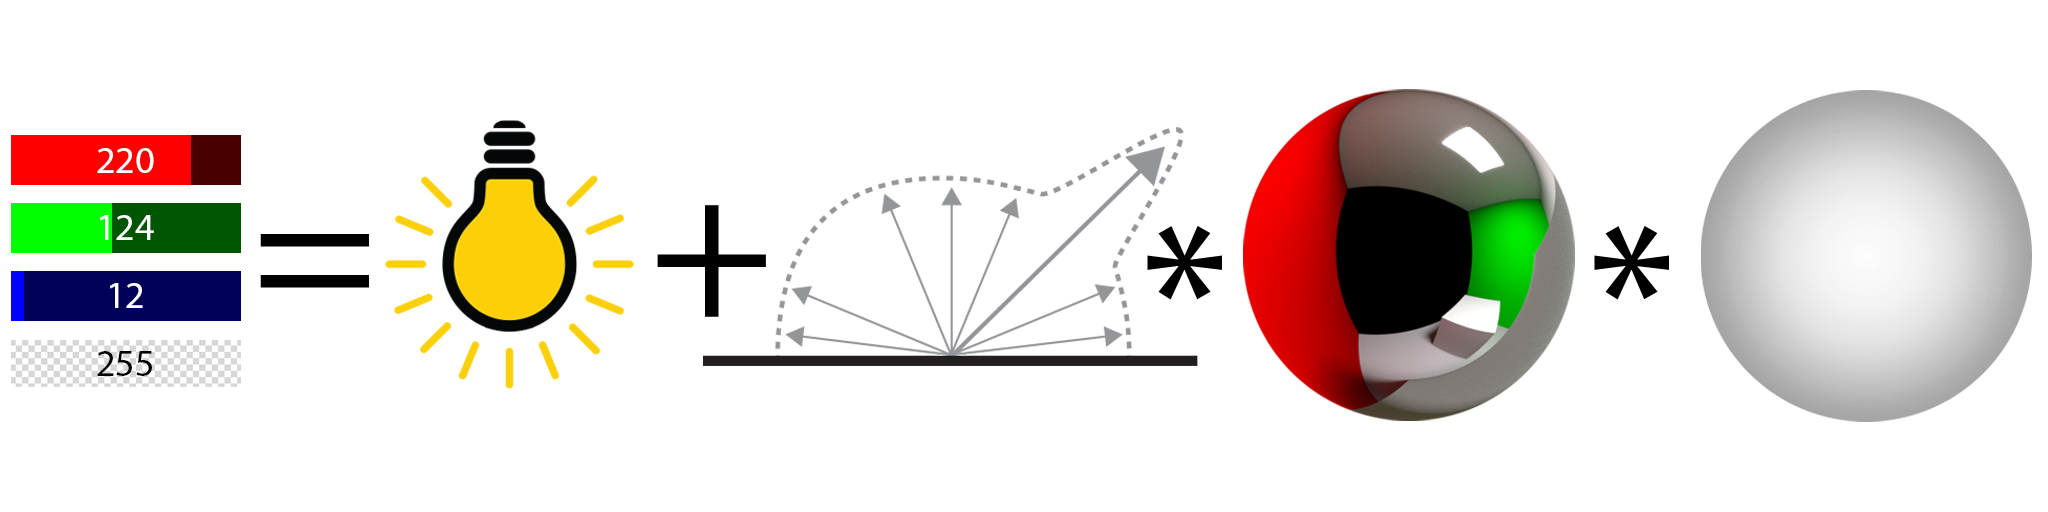
\includegraphics[width=0.9\textwidth]{img/rendering equation.png}
\end{frame}


\begin{frame}{Monte Carlo integrace}
\centering{Náhodné vzorkování $\times$ Diskrétní vzorkování}

\centering 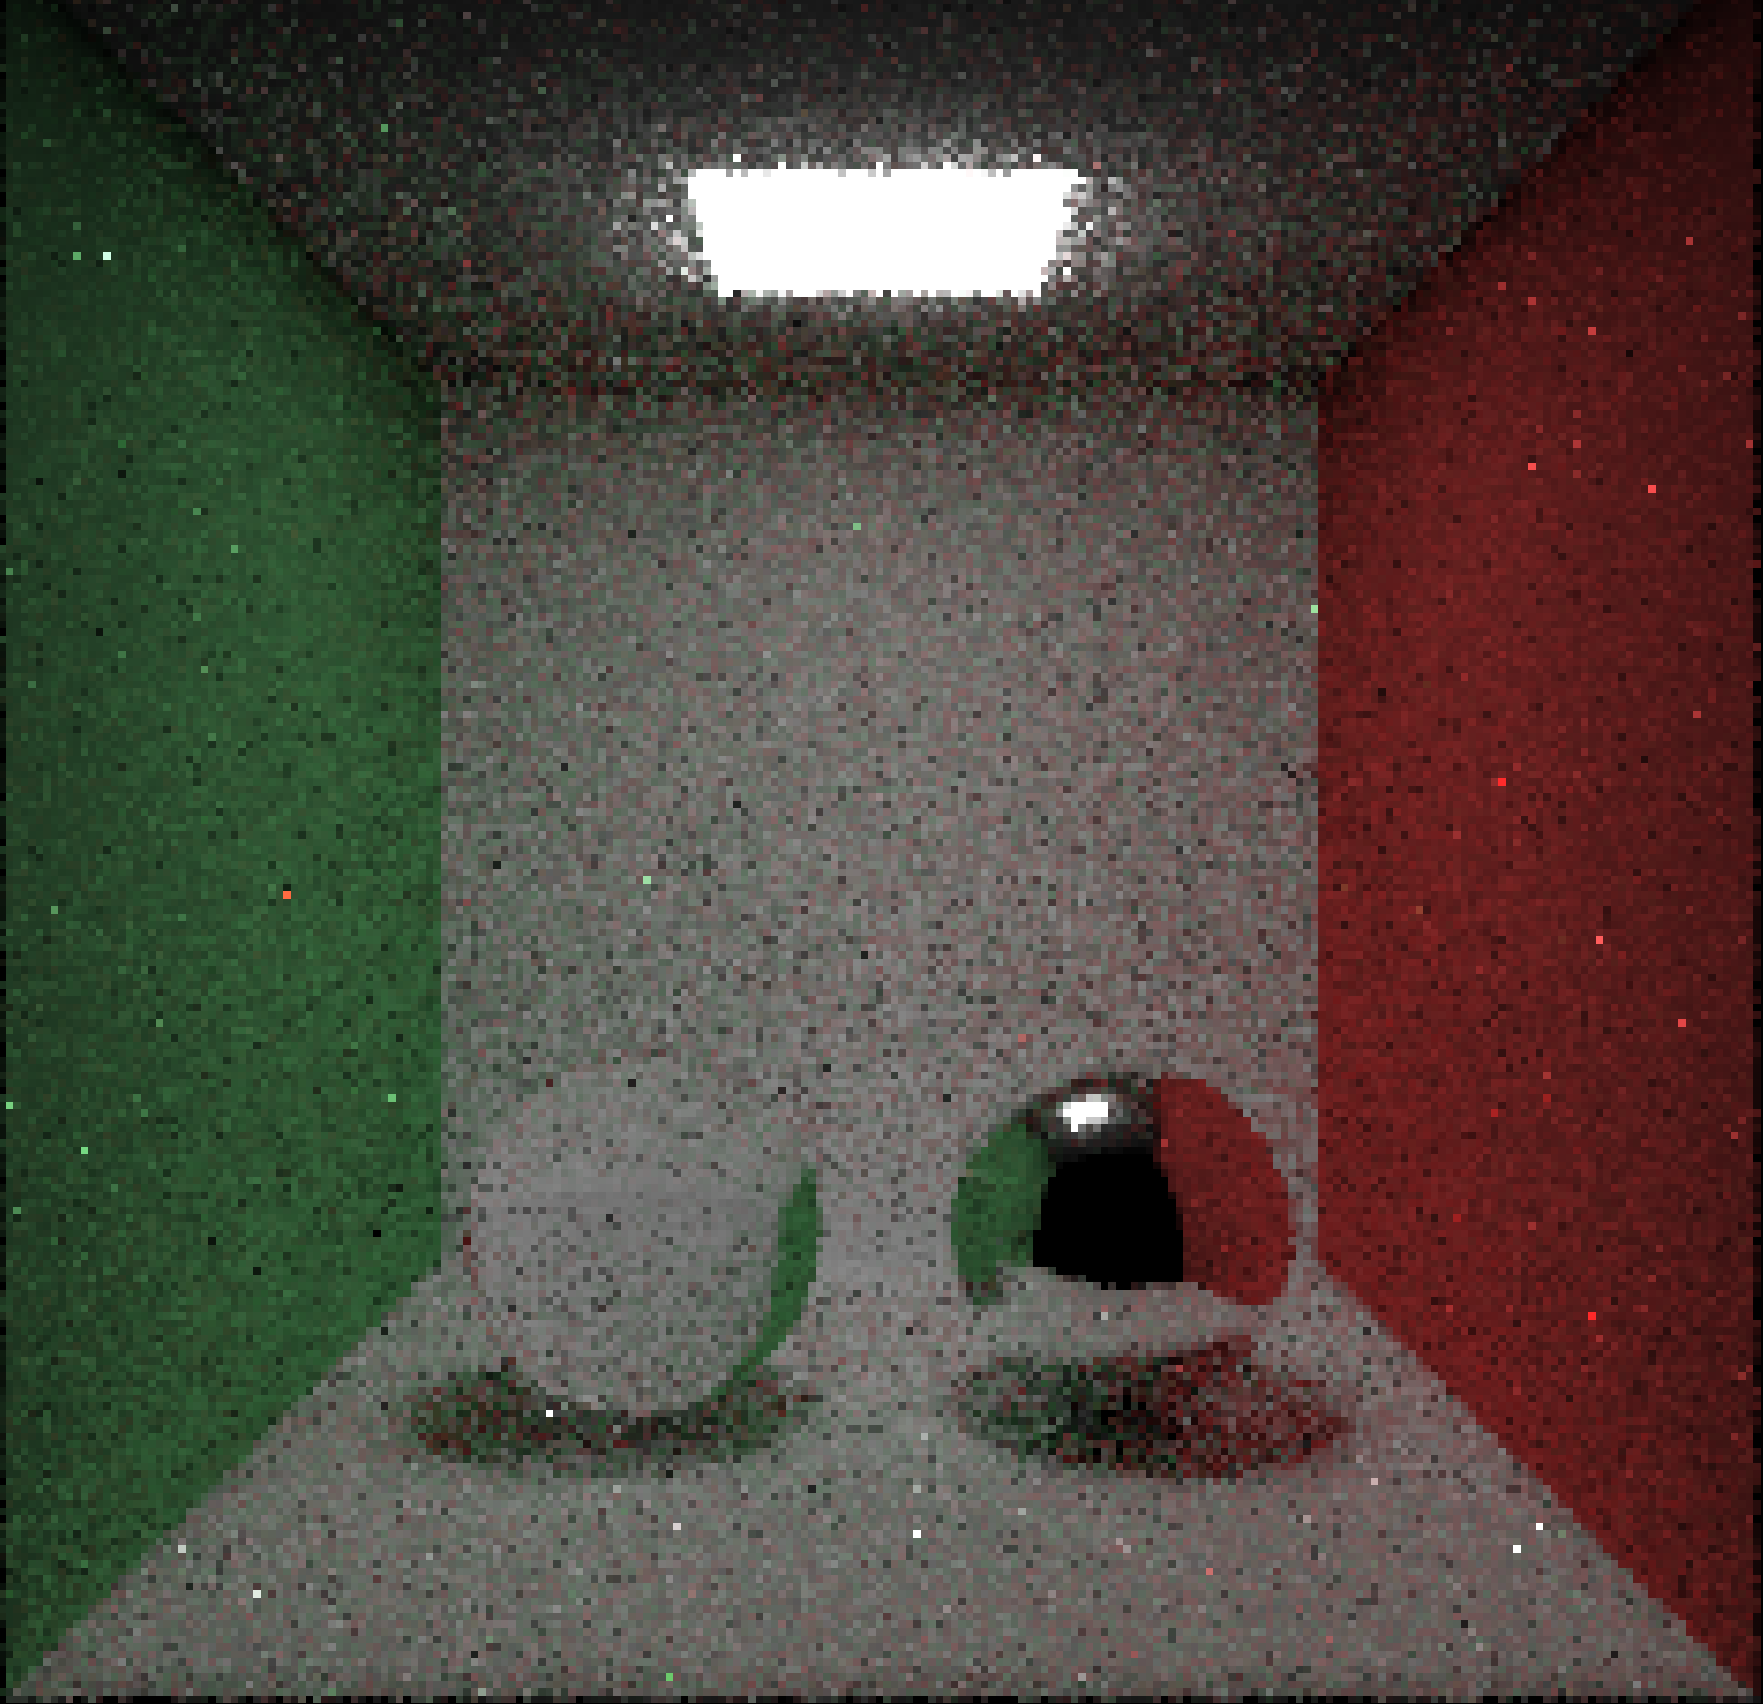
\includegraphics[width=0.4\textwidth]{img/MC sampling.png}
\centering 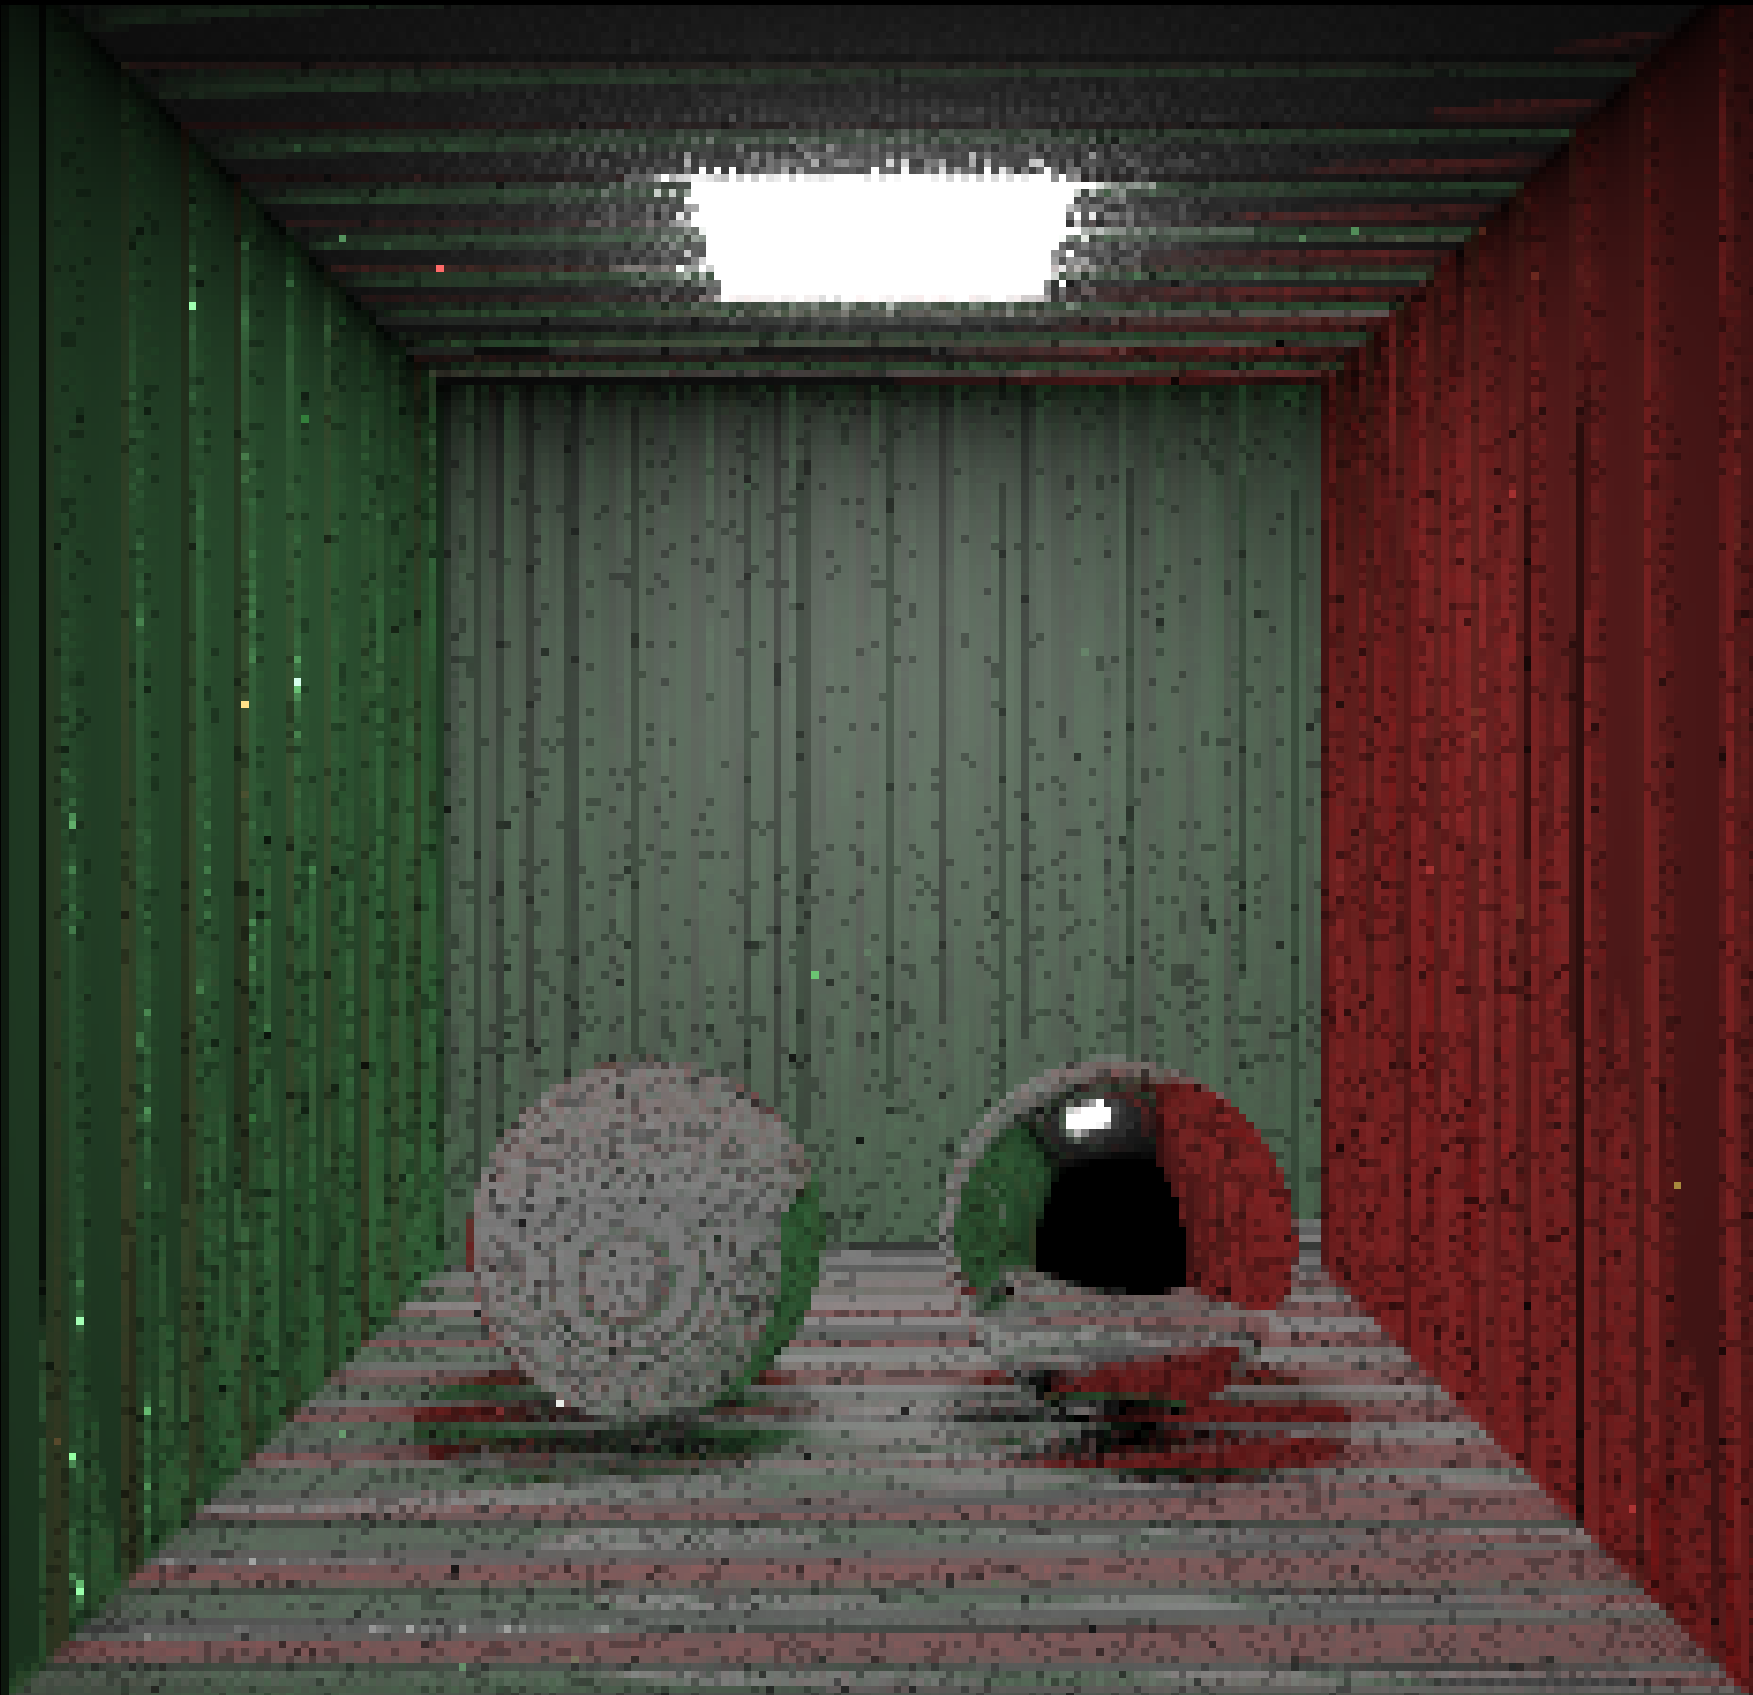
\includegraphics[width=0.4\textwidth]{img/discrete sampling.png}
\\
\centering 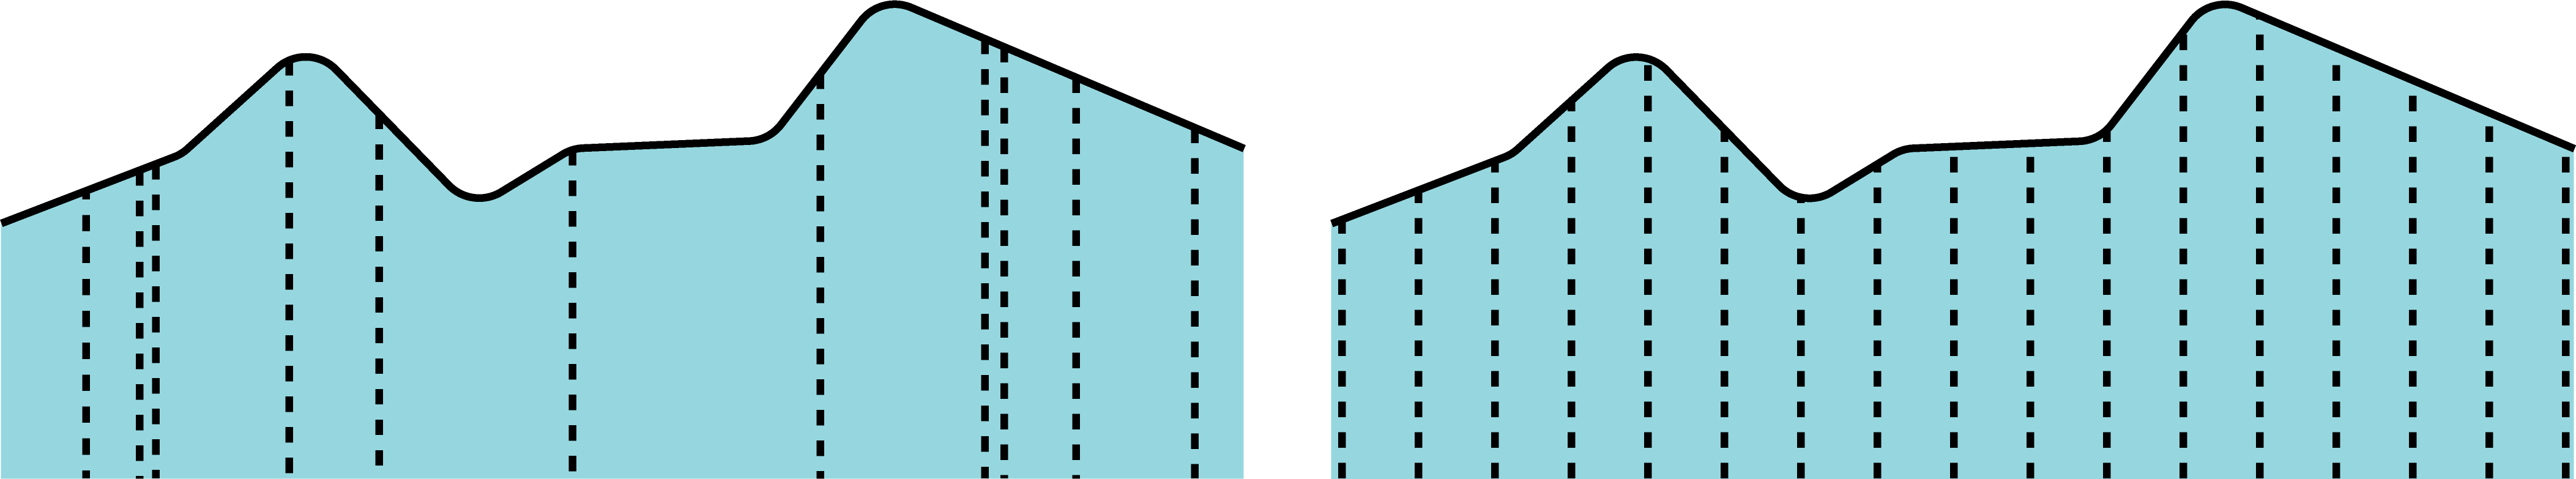
\includegraphics[width=0.9\textwidth]{img/monte carlo.png}
\end{frame}


\begin{frame}{Šum}
\begin{itemize}
  \item Od teď minimalizujeme šum a čas
\end{itemize}
\centering 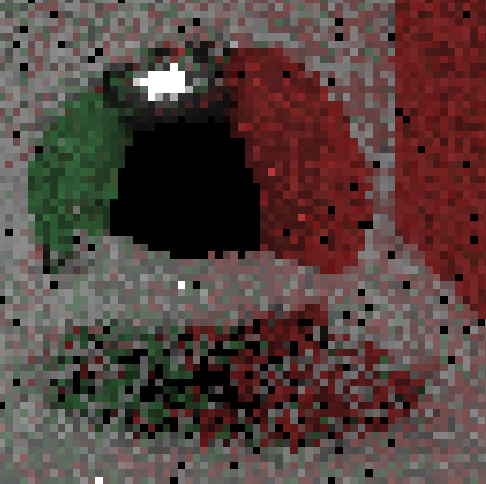
\includegraphics[width=0.4\textwidth]{img/1 sample.png}
\centering 
\includegraphics[width=0.386\textwidth]{img/1000 samples.png}
\\
\centering{\hspace{10pt} 1 paprsek na pixel \hspace{50pt} 1000 paprsků na pixel}
\end{frame}


\begin{frame}{Optimalizace šumu}
\begin{itemize}
  \item Tak náhodě trochu pomůžeme
  \item Přidáme paprsek ke světlu a náležitě to zprůměrujeme
\end{itemize}
\vfill
\centering 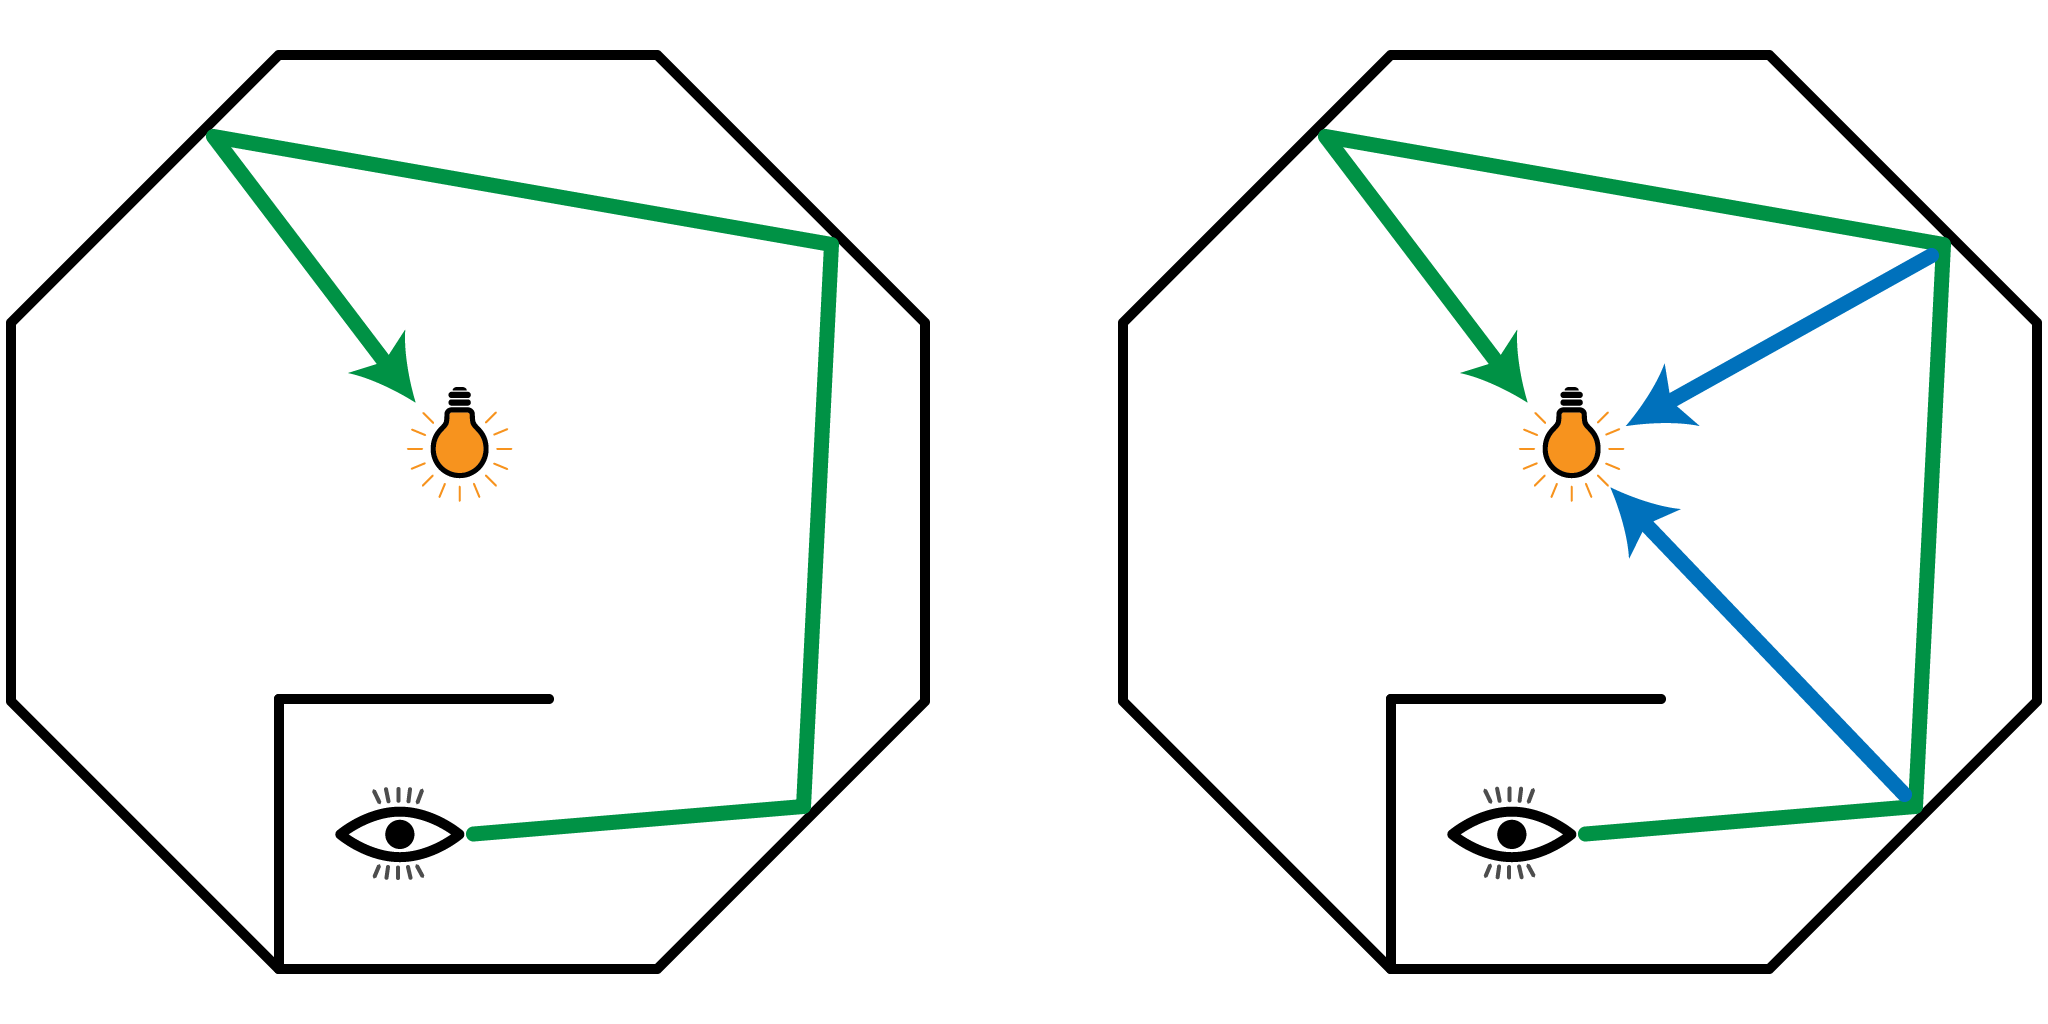
\includegraphics[width=0.8\linewidth]{img/light sampling.png}
\end{frame}


\begin{frame}{Kaustika}
\begin{itemize}
  \item Zaostřené světlo
  \item Materiály jako sklo, voda ...
\end{itemize}
\vfill
\centering 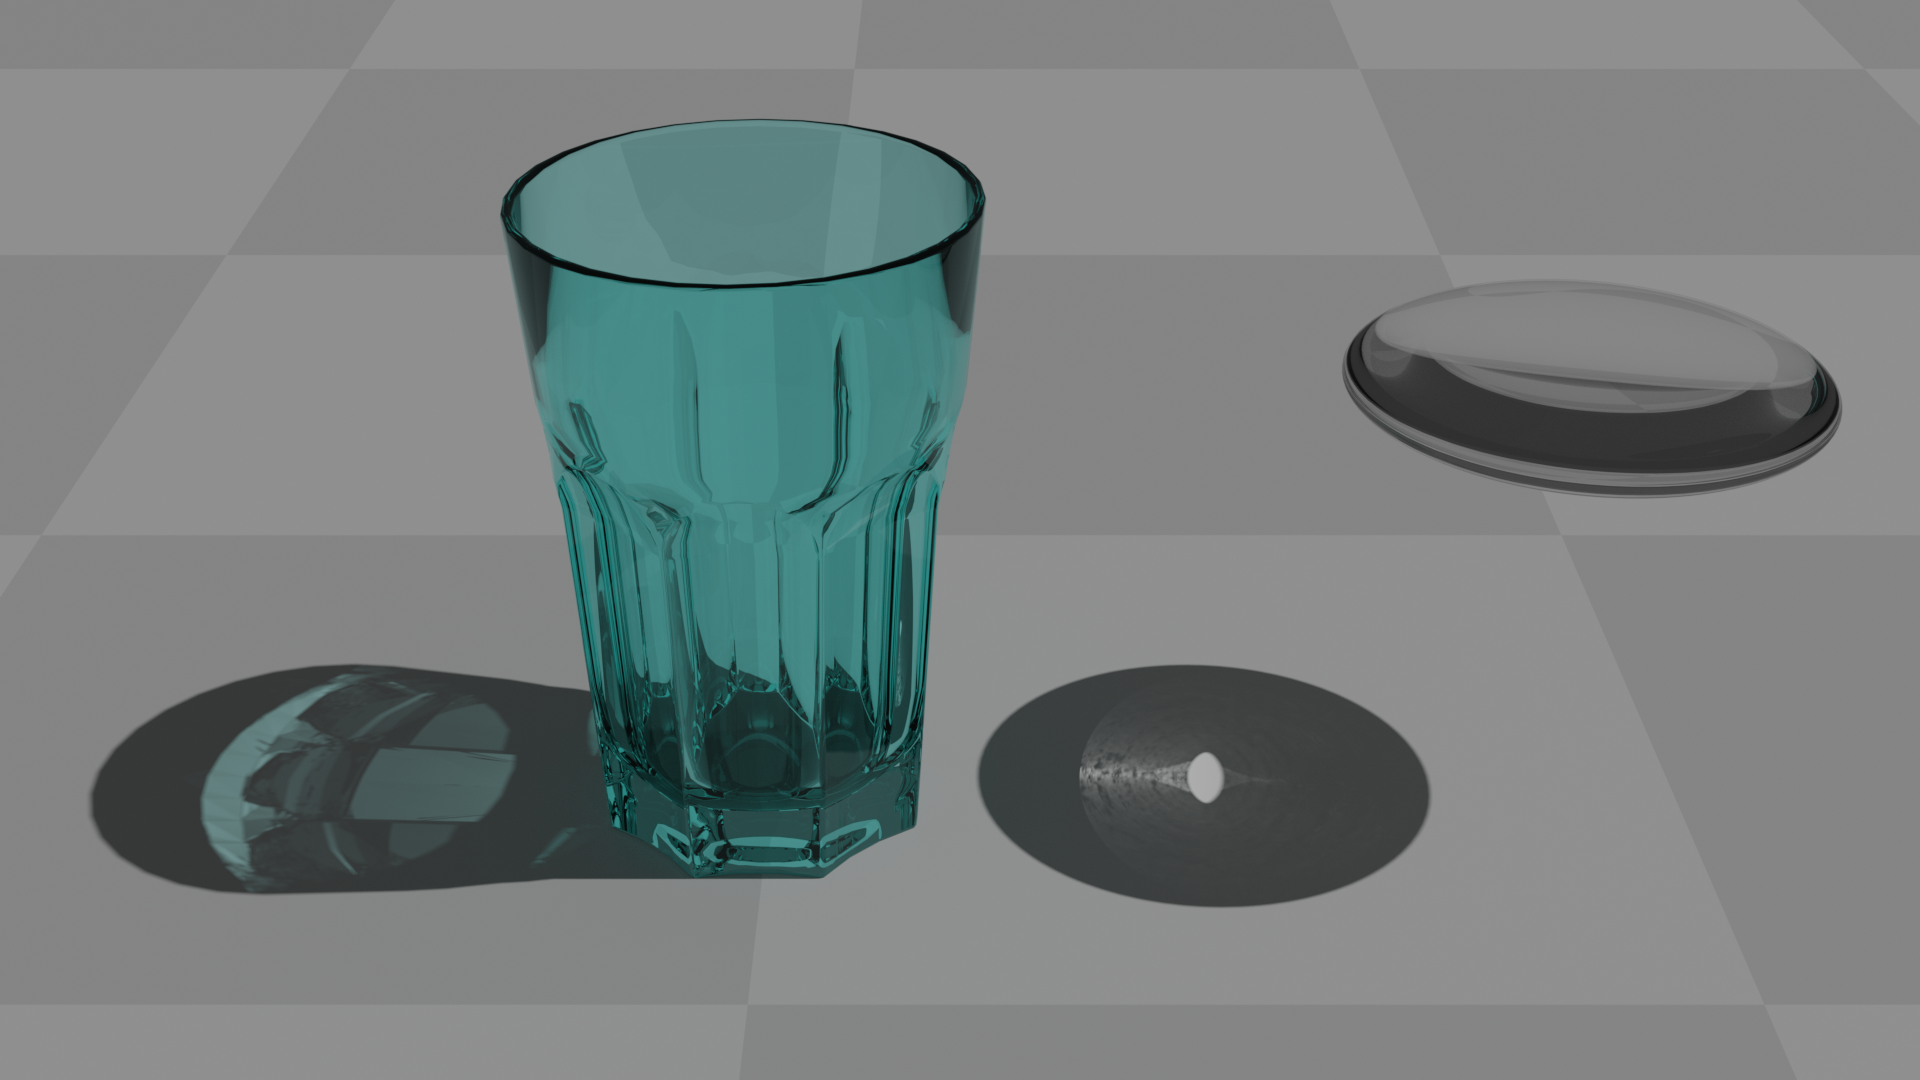
\includegraphics[width=0.5\textwidth]{img/caustics.png}
\end{frame}


\begin{frame}{Kaustika}
\centering 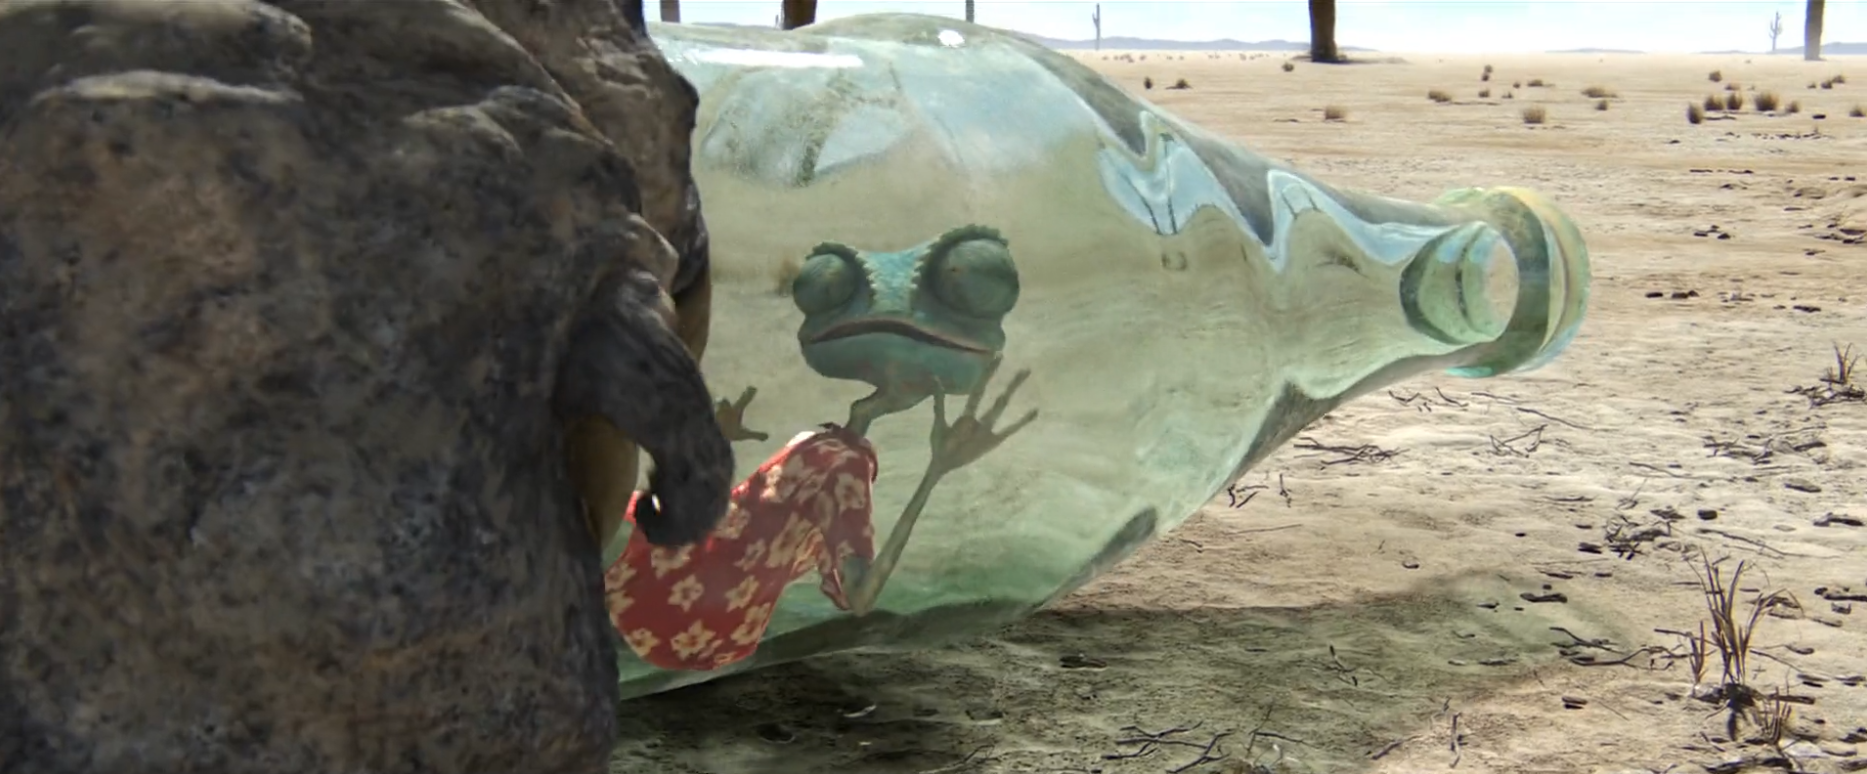
\includegraphics[width=0.95\textwidth]{img/rango.png}
\vfill
Pixar Rango (2011) (Zdroj: Disney Pixar)
\end{frame}


\begin{frame}{Obousměrné trasování cesty}
\begin{itemize}
  \item Najednou nám vzorkování světla nefunguje
\end{itemize}
\vfill
\centering 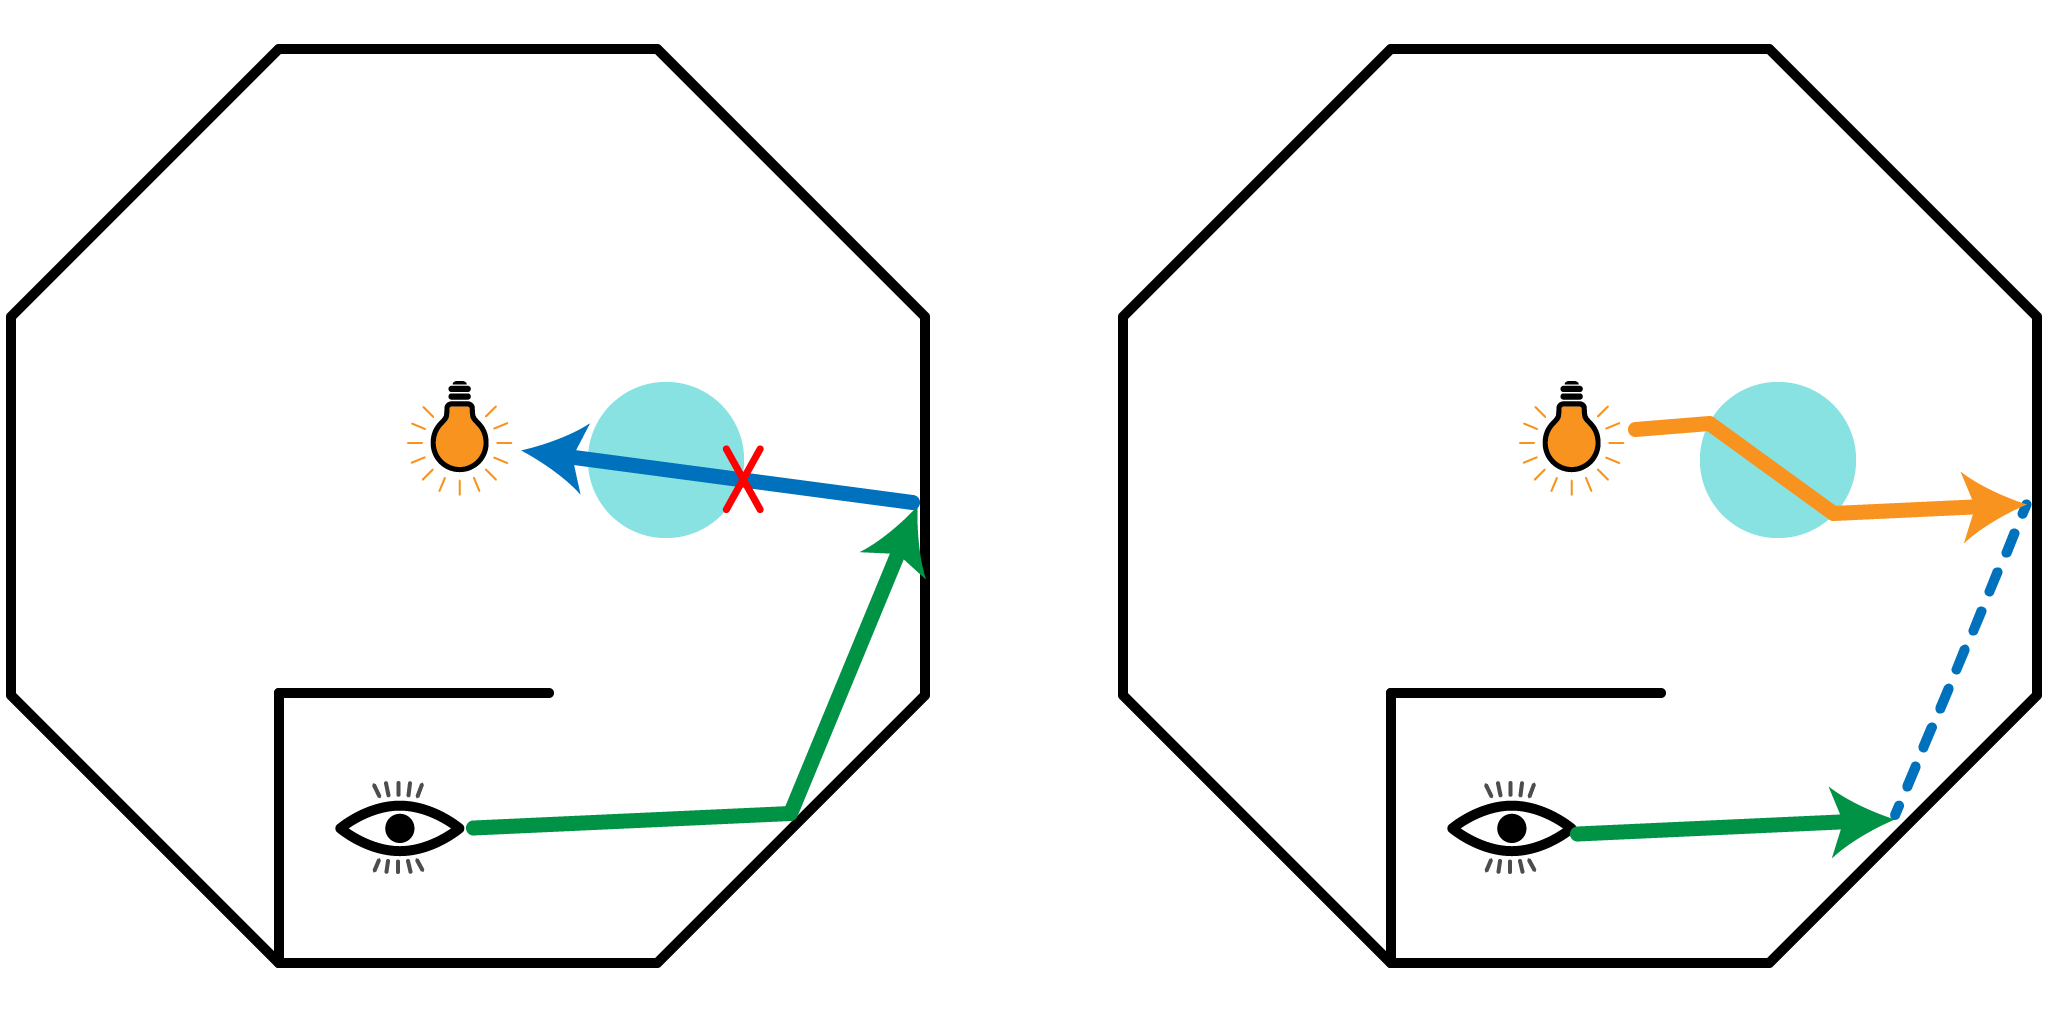
\includegraphics[width=0.8\linewidth]{img/bidirectional scene.png}
\vfill
\centering 
\includegraphics[width=0.7\textwidth]{img/bidirectional.png}
\end{frame}


\begin{frame}{BRDF}
Bidirectional Reflectance Distribution Function
\begin{itemize}
  \item \textbf{Diffuse}: matný povrch
  \item \textbf{Mirror}: ostrý odraz
  \item \textbf{Glossy}: rozostřený odraz
\end{itemize}
\vfill
\centering 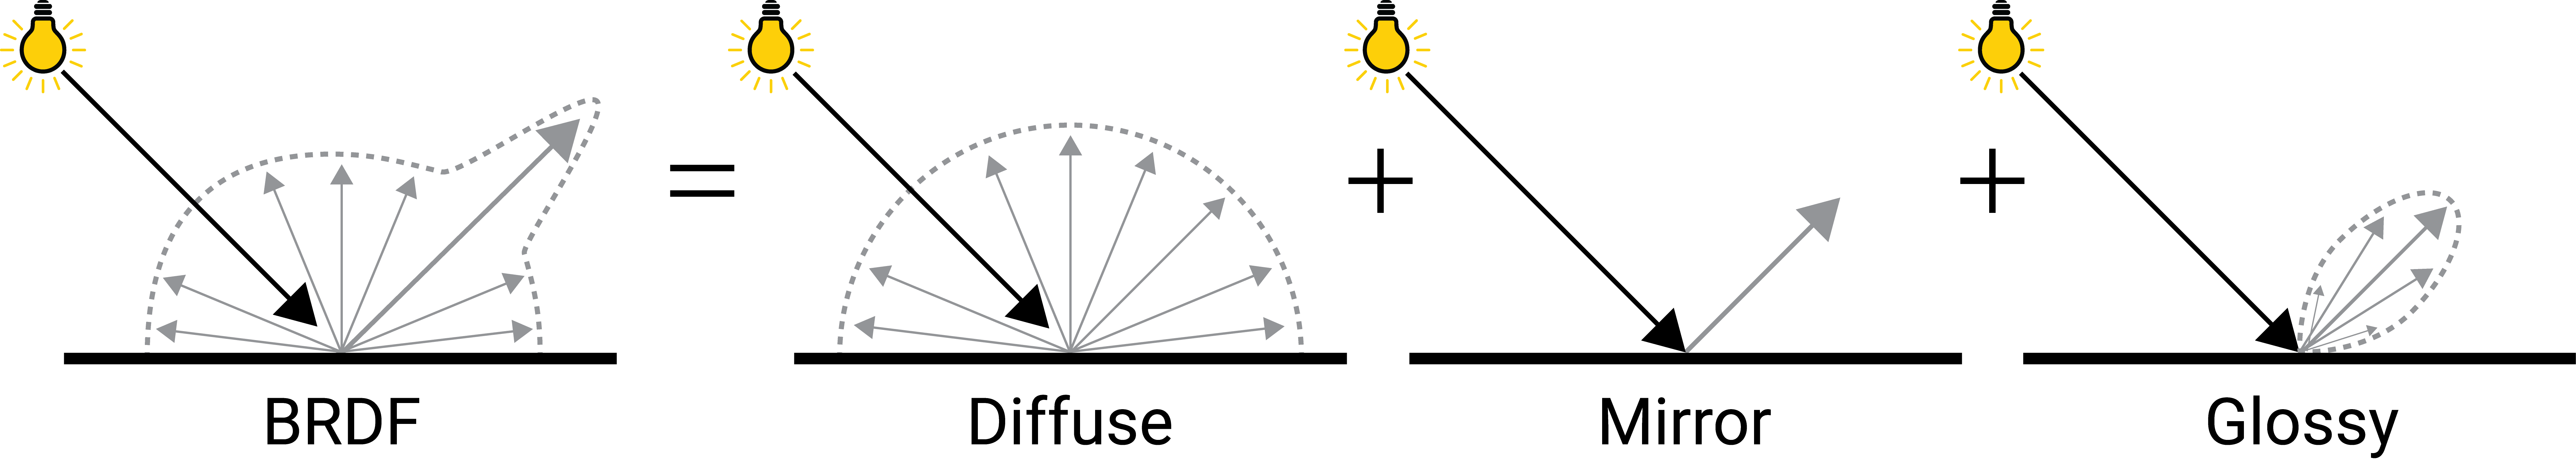
\includegraphics[width=1.0\textwidth]{img/brdf.png}
\end{frame}


\begin{frame}{BRDF}
Různé drsnosti materiálu
\vfill
\centering 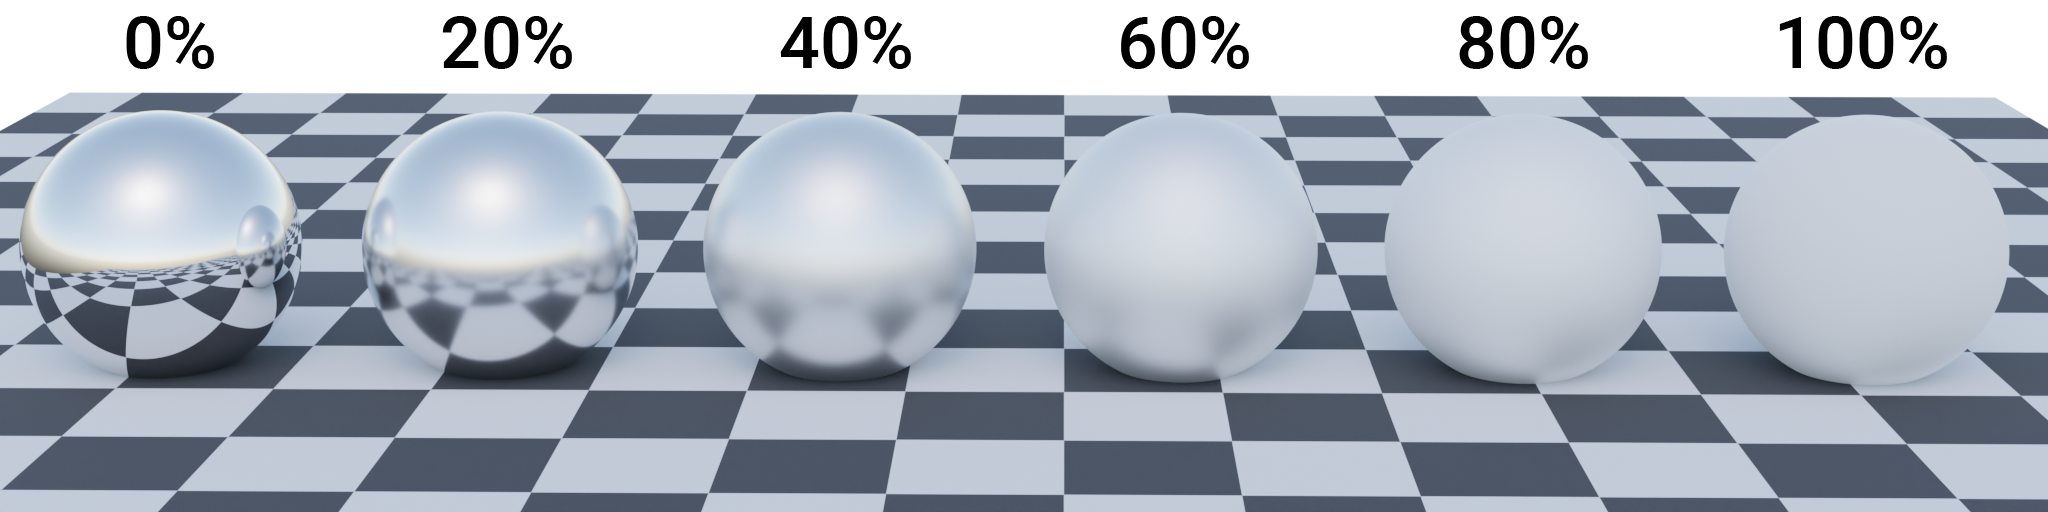
\includegraphics[width=1\textwidth]{img/roughness.png}
\end{frame}


\begin{frame}{Měření BRDF}
\begin{itemize}
  \item Matematicky hezký, ale jak to změřit
\end{itemize}
\vfill
\centering 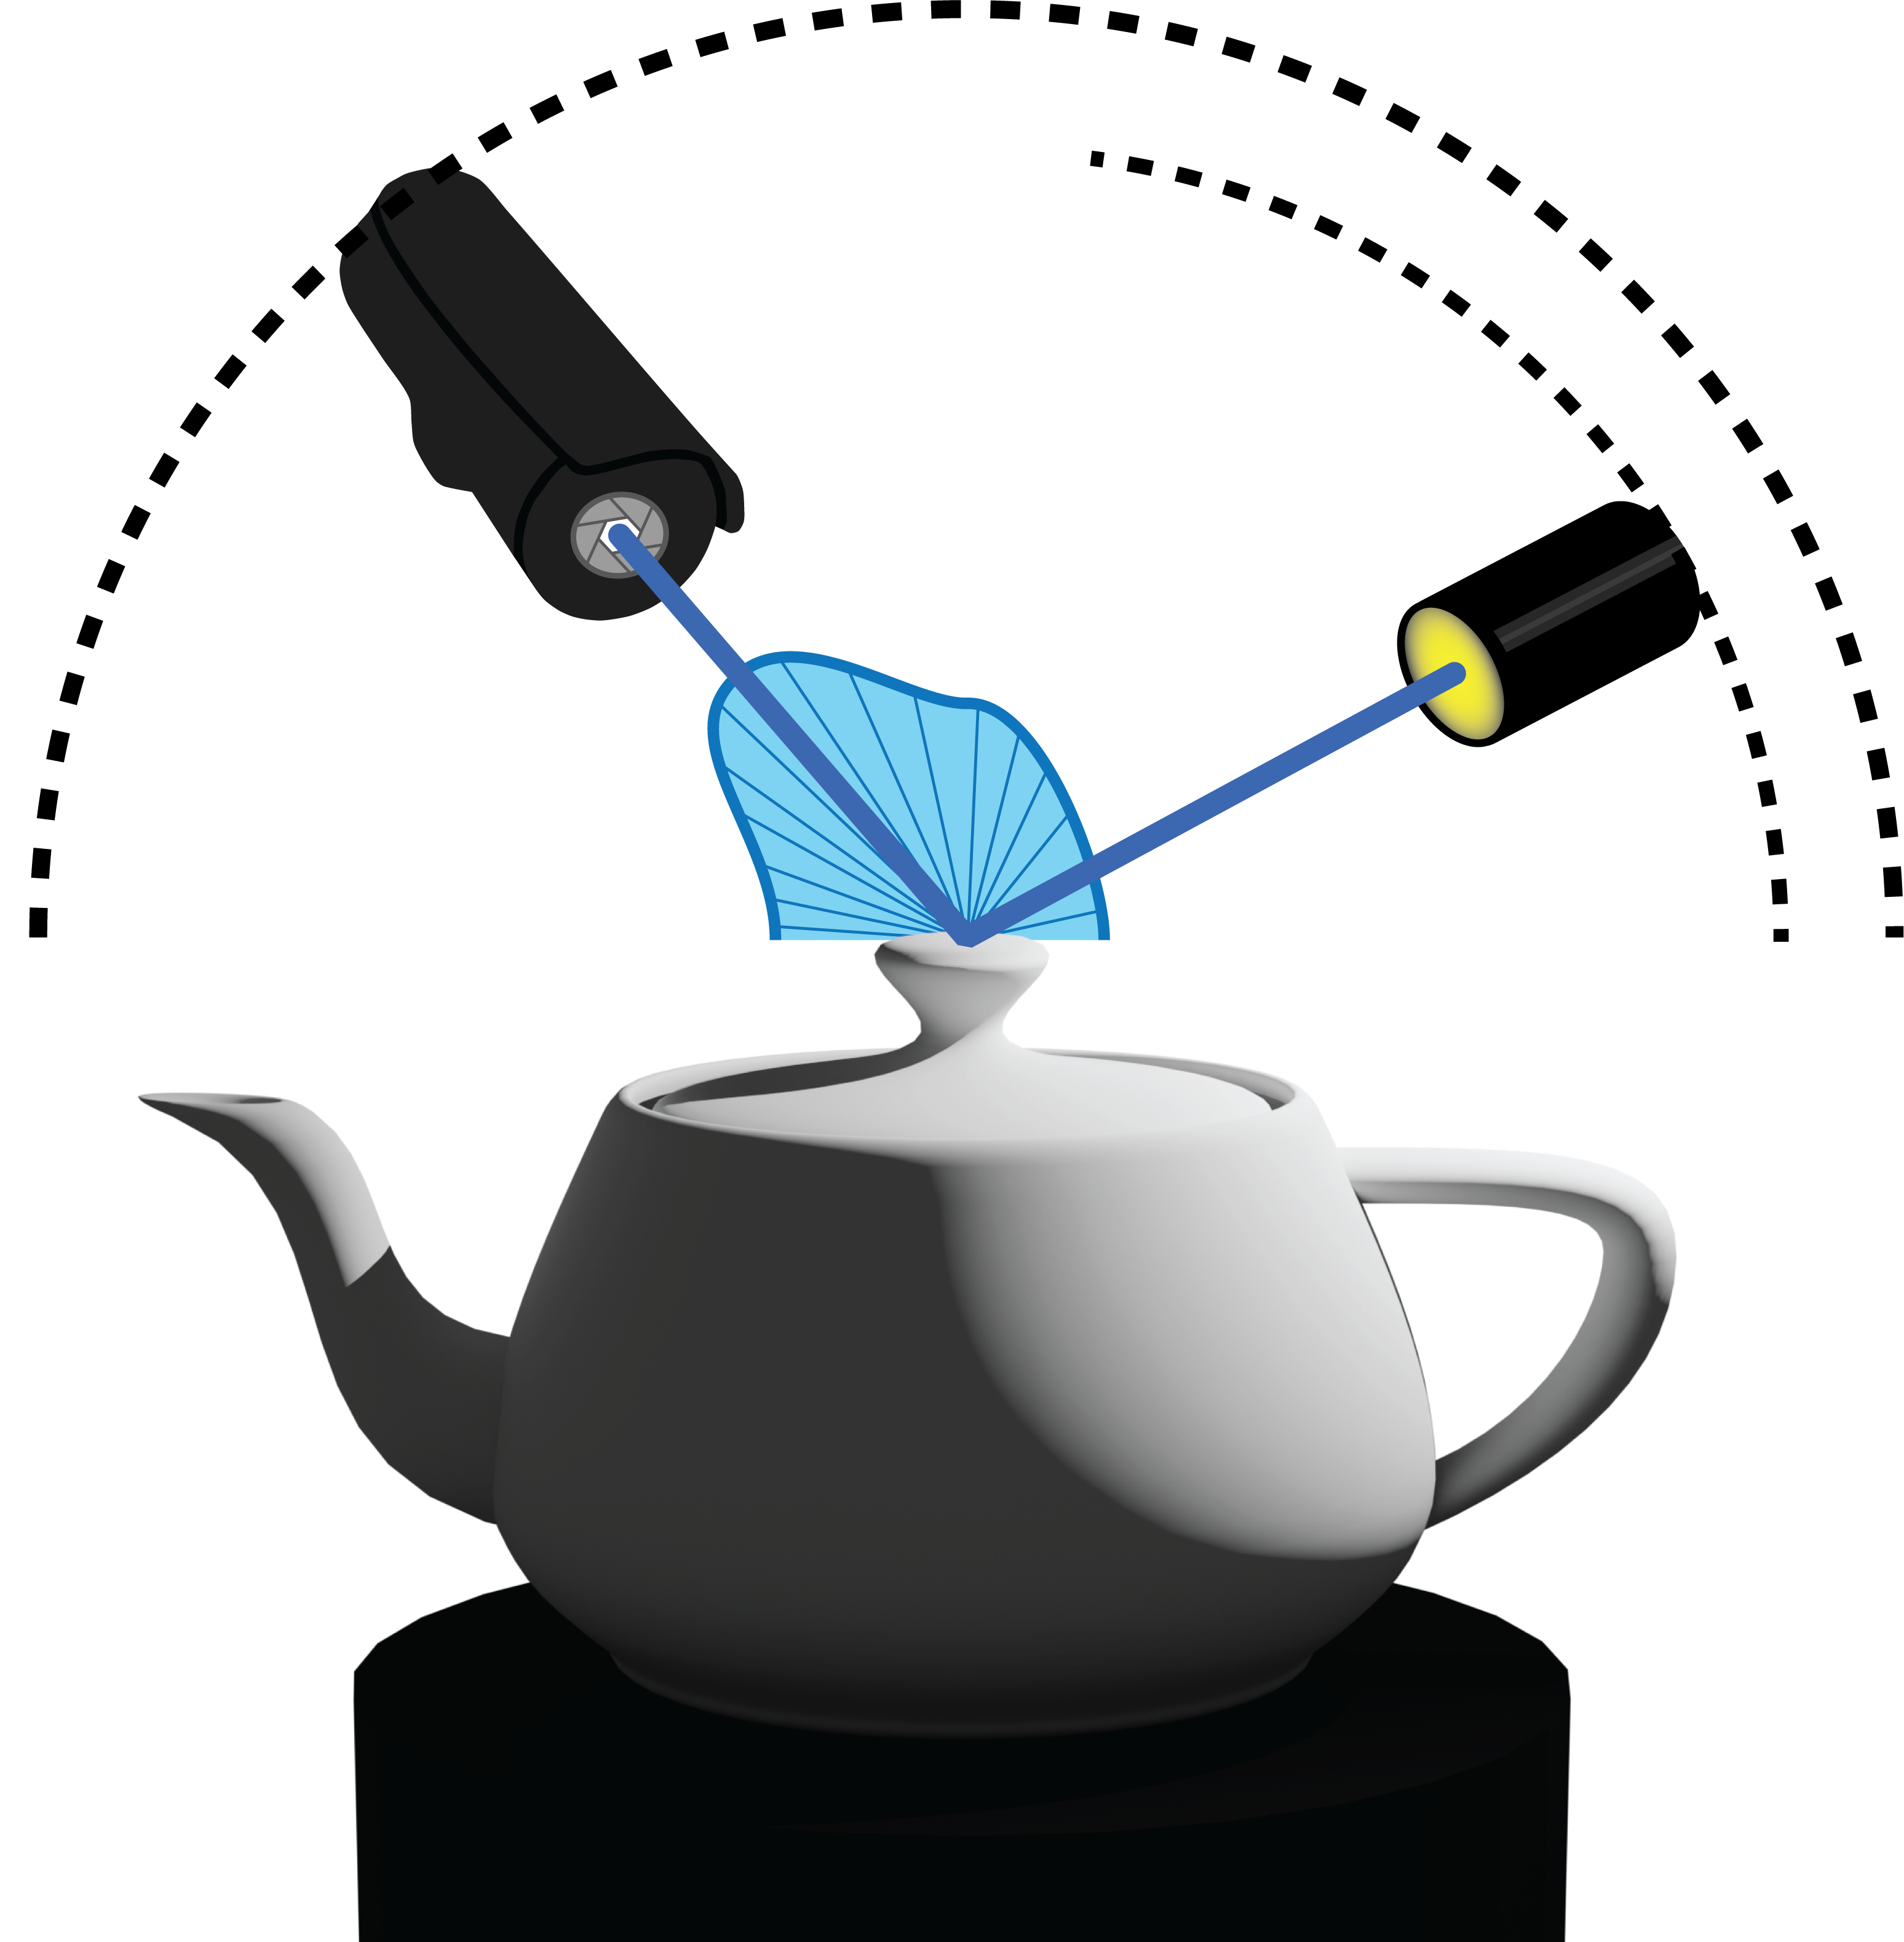
\includegraphics[width=.6\textwidth]{img/measuring brdf.png}
\end{frame}


\begin{frame}{BRDF vzorkování}
\begin{itemize}
  \item A zase nám vzorkování světla nefunguje 
  \item Malá šance se trefit (takže té šanci budeme muset zase pomoct)
\end{itemize}
\vfill
\centering 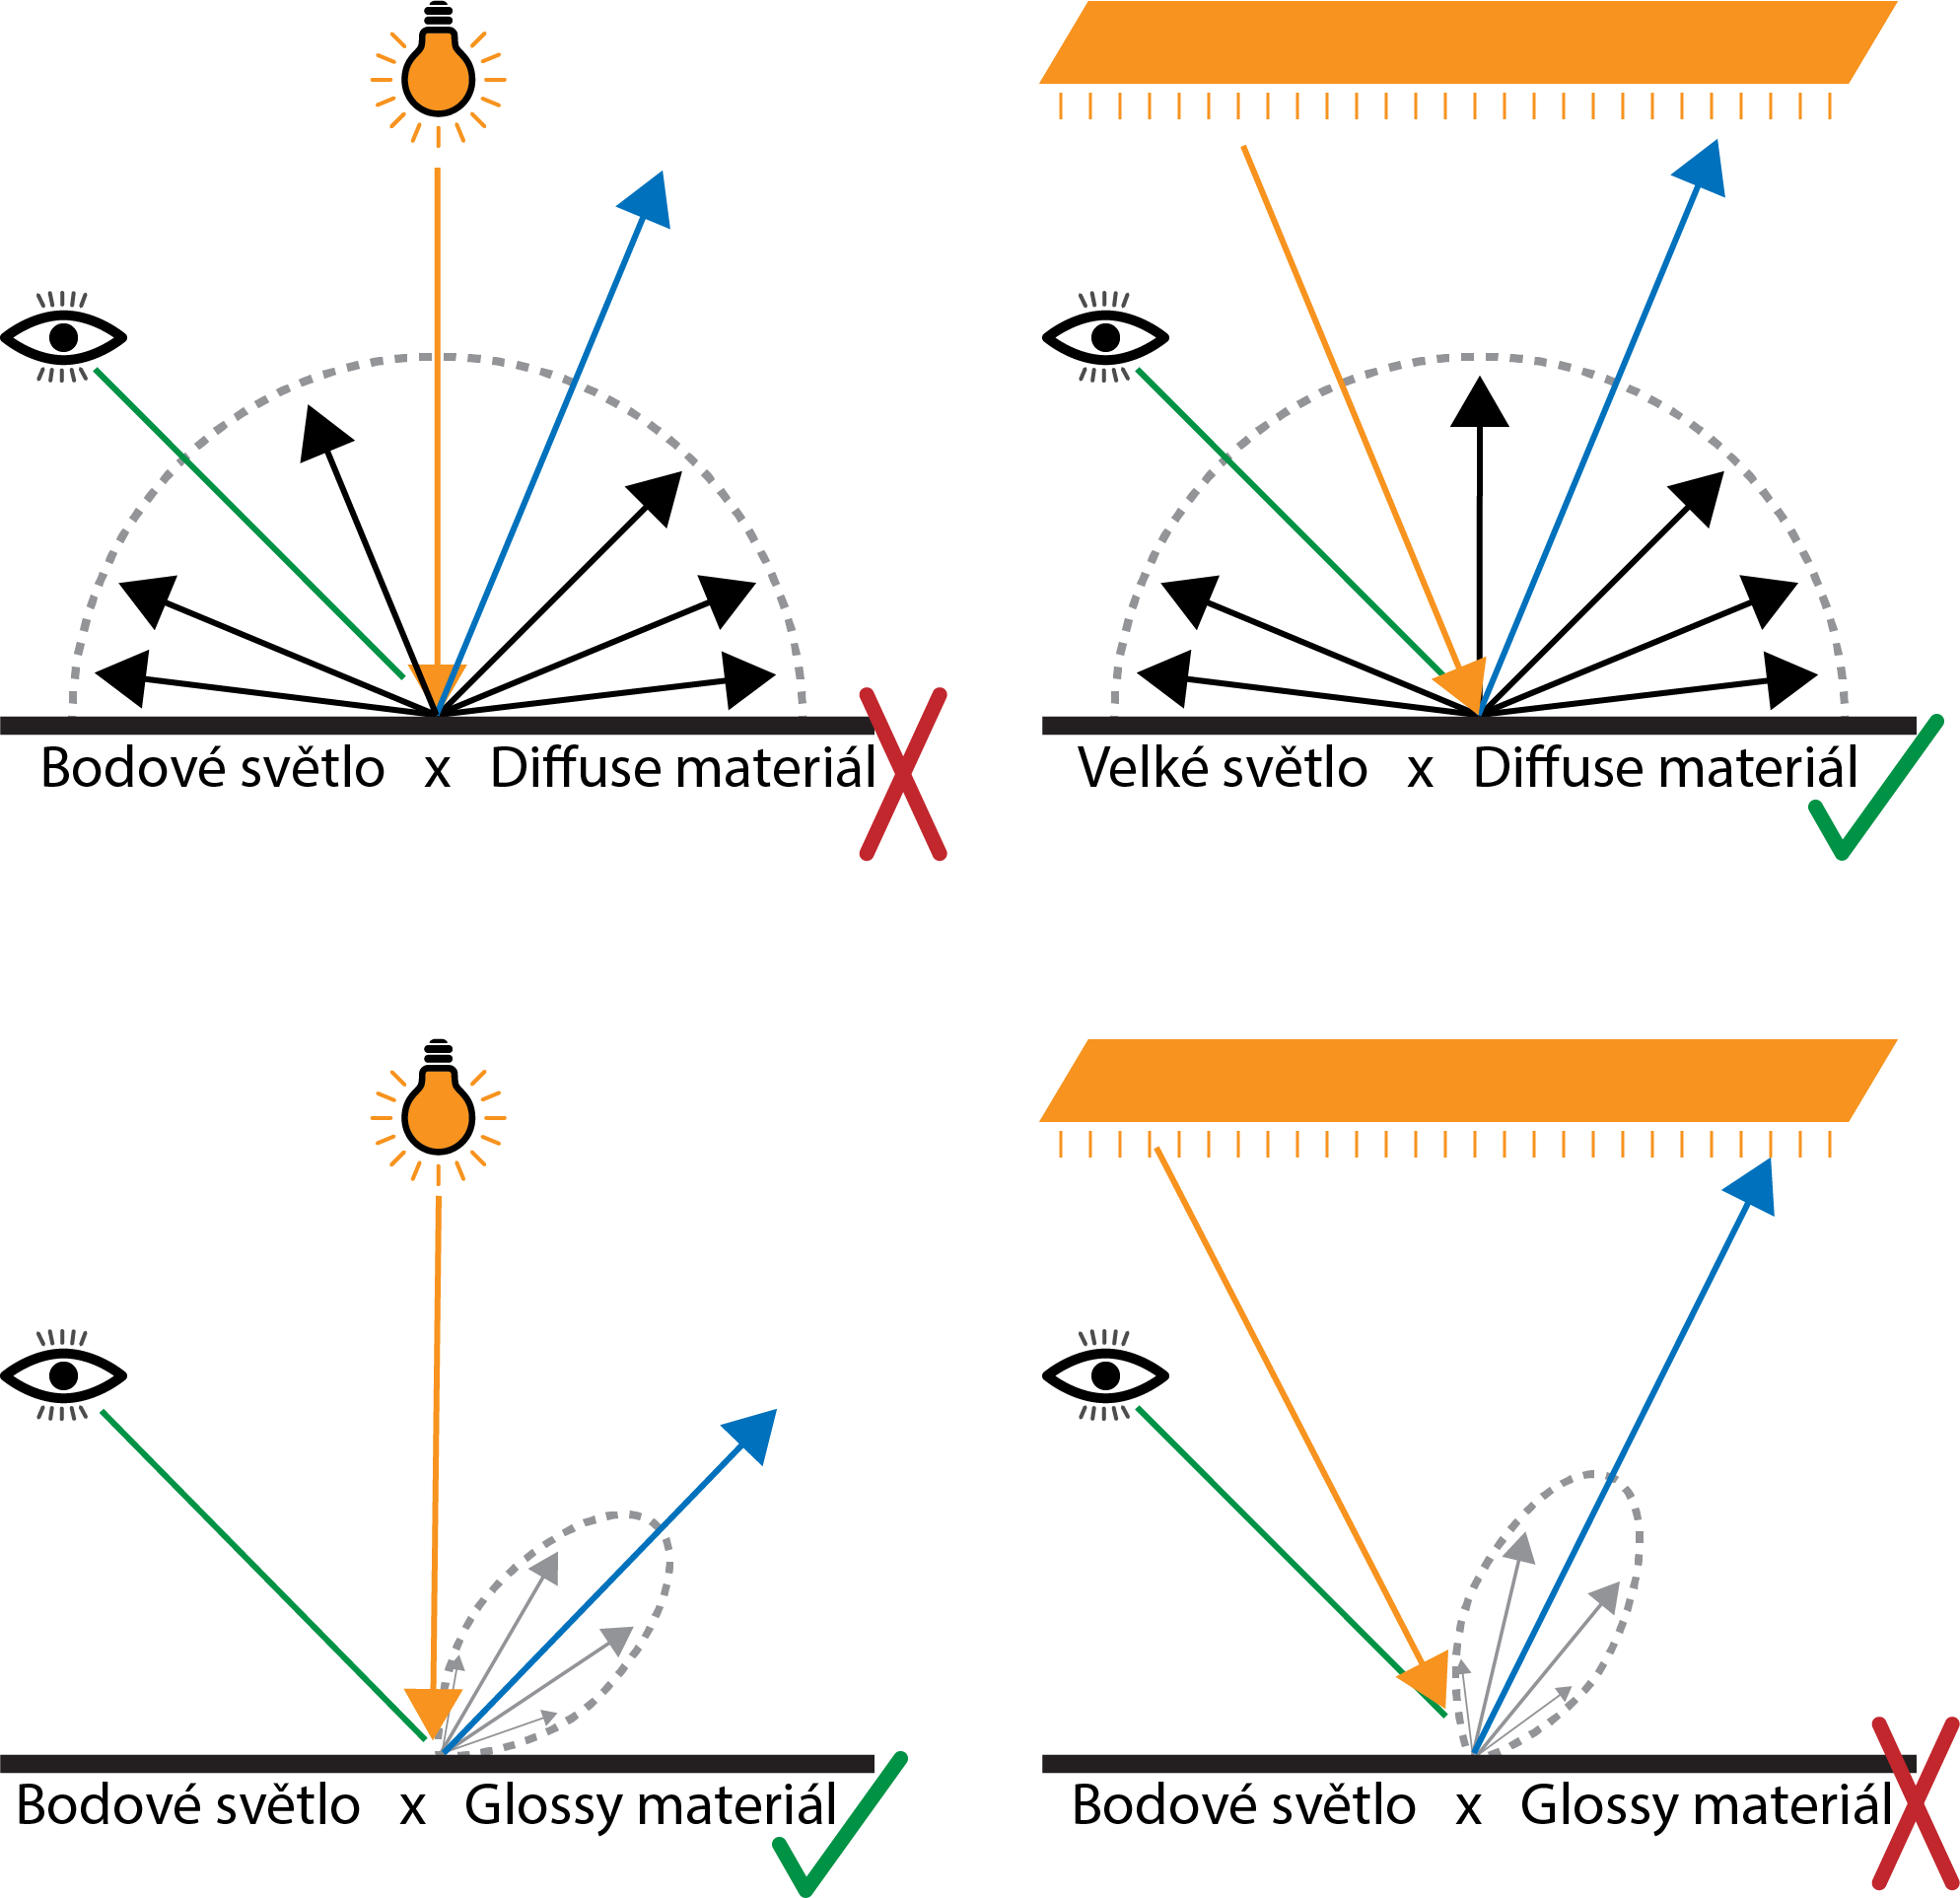
\includegraphics[width=0.5\linewidth]{img/sampling strategies.png}
\end{frame}


\begin{frame}{MIS}
\begin{itemize}
  \item Multiple Importance Sampling
\end{itemize}
\vfill
\centering{
$
v_{\text{světlo}}(\omega) = \frac{p_{\text{světlo}}(\omega)}
{p_{\text{světlo}}(\omega)^{\beta} + p_{\text{brdf}}(\omega)}
$
\hskip 10pt
$
v_{\text{brdf}}(\omega)  = \frac{p_{\text{brdf}}(\omega)}
{p_{\text{světlo}}(\omega)^{\beta} + p_{\text{brdf}}(\omega)}.
$
}
\vfill
\centering 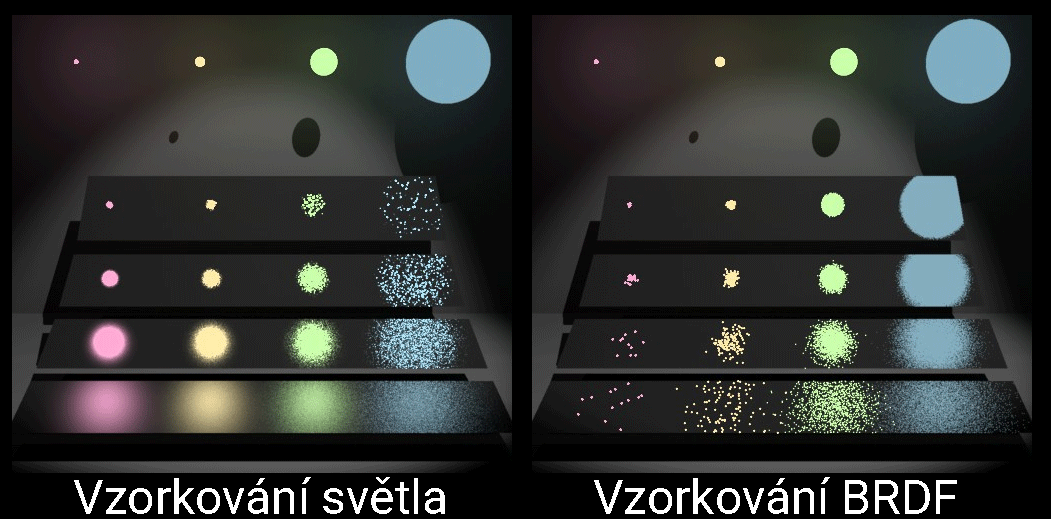
\includegraphics[width=.7\textwidth]{img/mis.png}\\
{\footnotesize \hfill Img source: Eric Veach}
\end{frame}


\begin{frame}{MIS}
\begin{itemize}
  \item Vyvážená kombinace strategií
\end{itemize}
\vfill
\centering 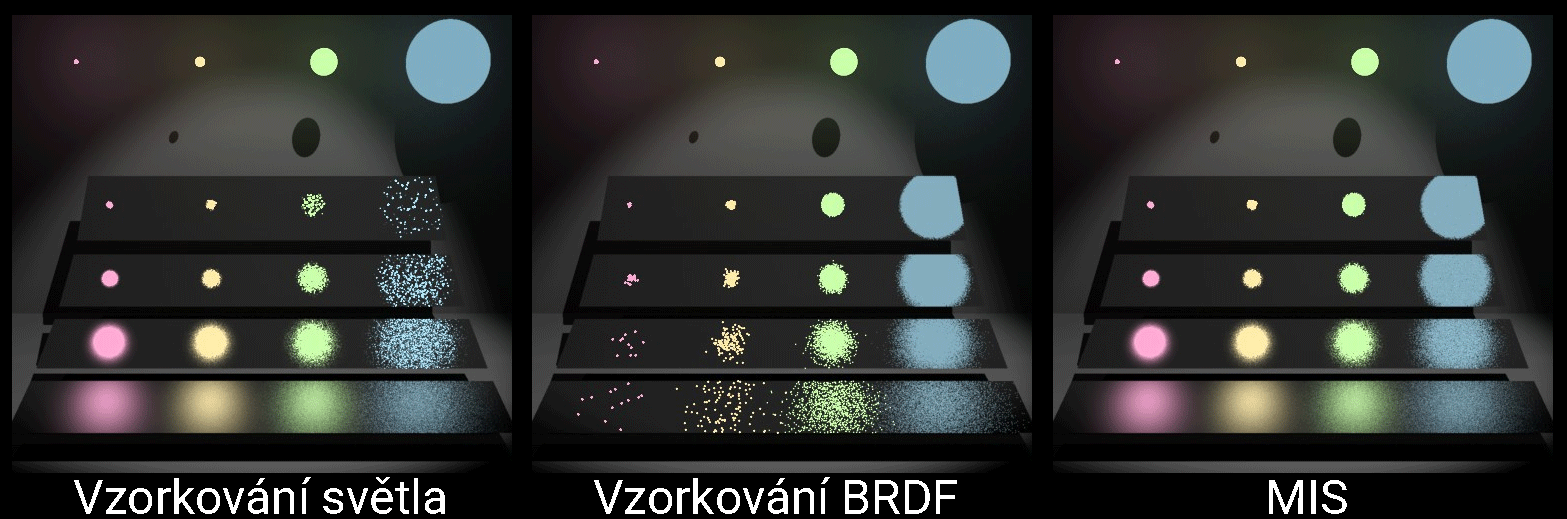
\includegraphics[width=1\textwidth]{img/mis - full.png}\\
{\footnotesize \hfill Img source: Eric Veach}
\end{frame}



\begin{frame}{Speciální jevy}
\begin{itemize}
  \item Mikrofacety: drsnost, mlha
  \item Subsurface scattering: průsvitné materiály
\end{itemize}
\vfill
\centering 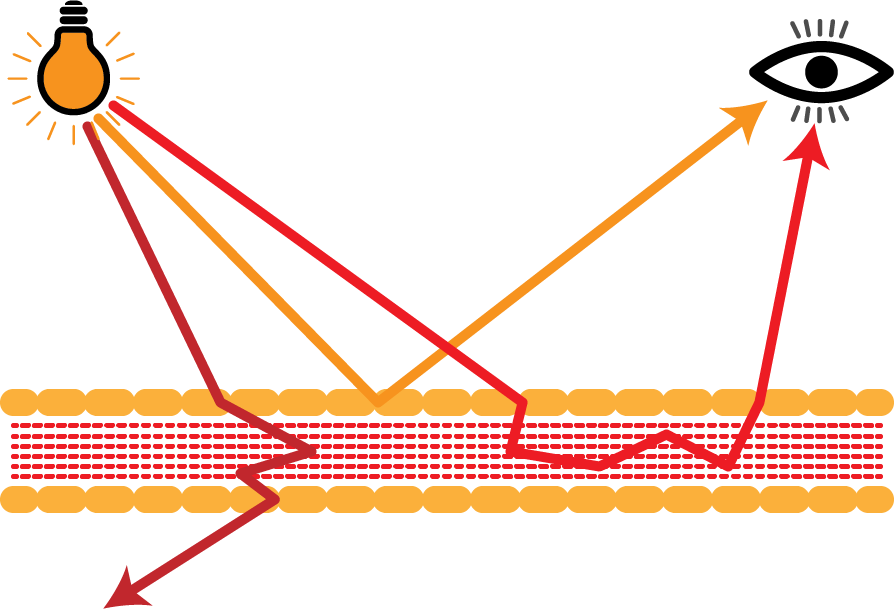
\includegraphics[width=0.7\textwidth]{img/subsurface scatering.png}
\end{frame}


\begin{frame}{Datové struktury}
\begin{itemize}
  \item $O(n)$ by bylo na dlouho
  \item Chceme $O(\log{n})$ 
\end{itemize}
\centering 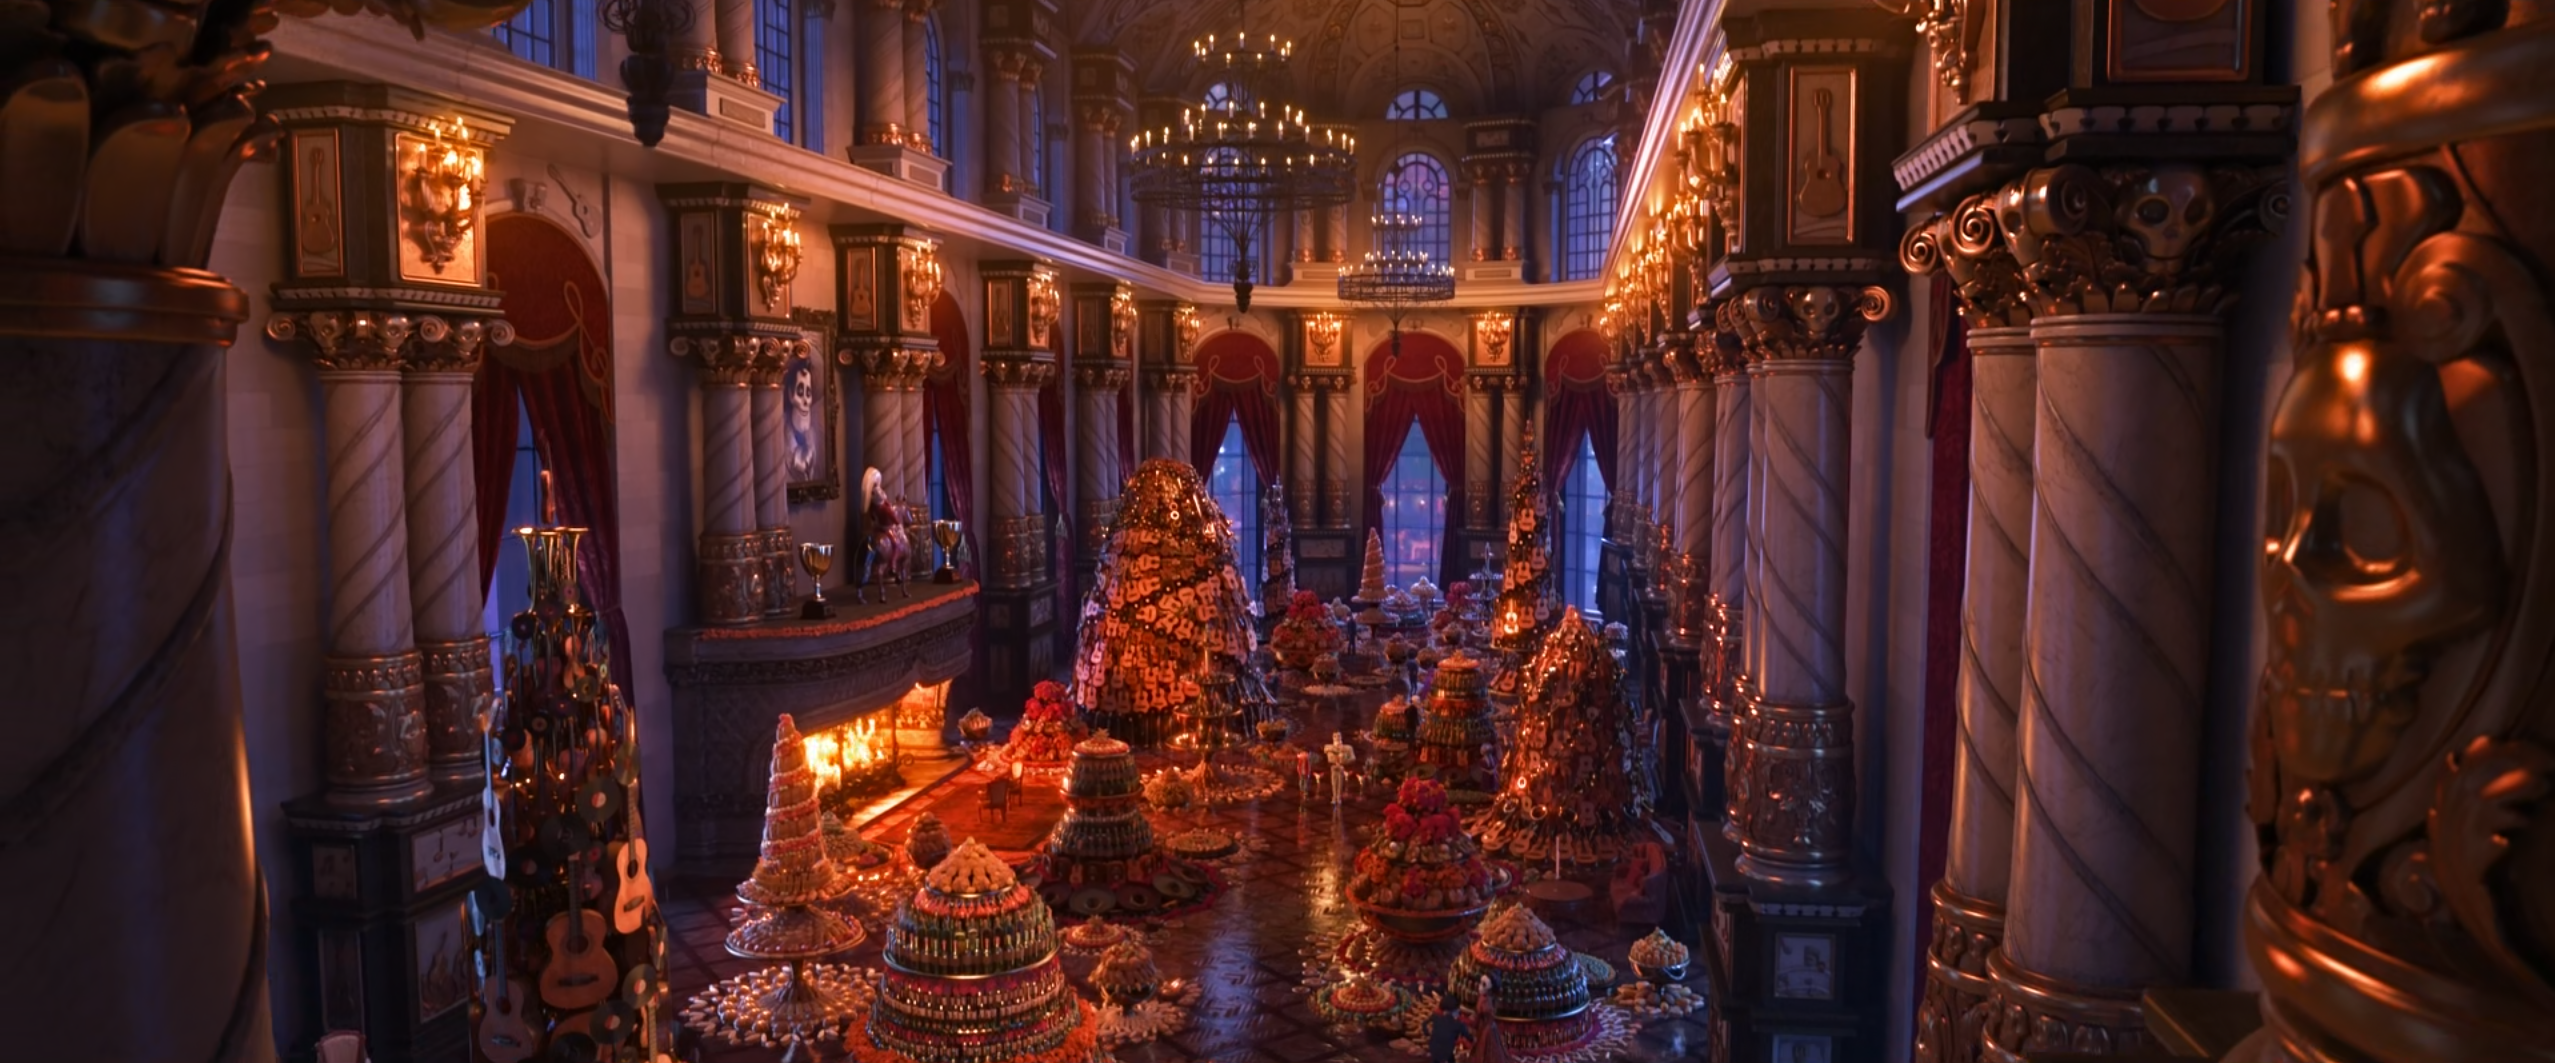
\includegraphics[width=1\textwidth]{img/coco.png}
{\footnotesize \hfill Film Coco: 20 milionů objektů (Zdroj Disney Pixar)}
\end{frame}


\begin{frame}{Datové struktury}
\begin{itemize}
  \item BVH (bounding volume hierarchy)
    \begin{itemize}
        \item AABB (Axis-aligned bounding boxes)
    \end{itemize}
  \item Vytvoření: $O(n \log{n})$
  \item Vyhledávání: $O(\log{n})$
\end{itemize}
\centering 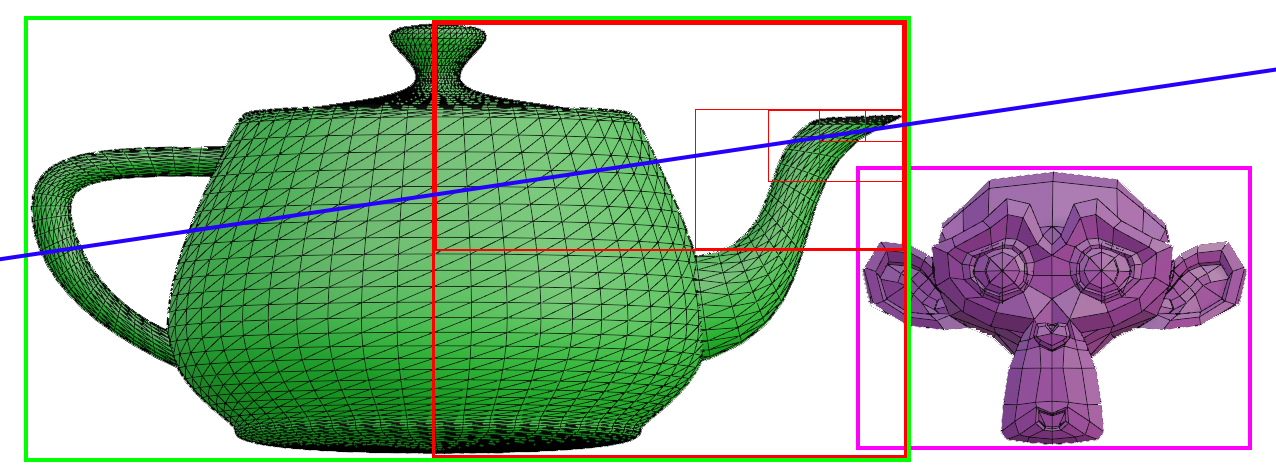
\includegraphics[width=.95\textwidth]{img/bvh.png}
\end{frame}


\begin{frame}{Efekty kamery}
Věci které máme témeř zdarma
\begin{itemize}
  \item \textbf{Anti-aliasing: více paprsků/pixel}
  \item Depth of field: simulace clony
  \item Motion blur: čas jako další rozměr
\end{itemize}
\vfill
\centering 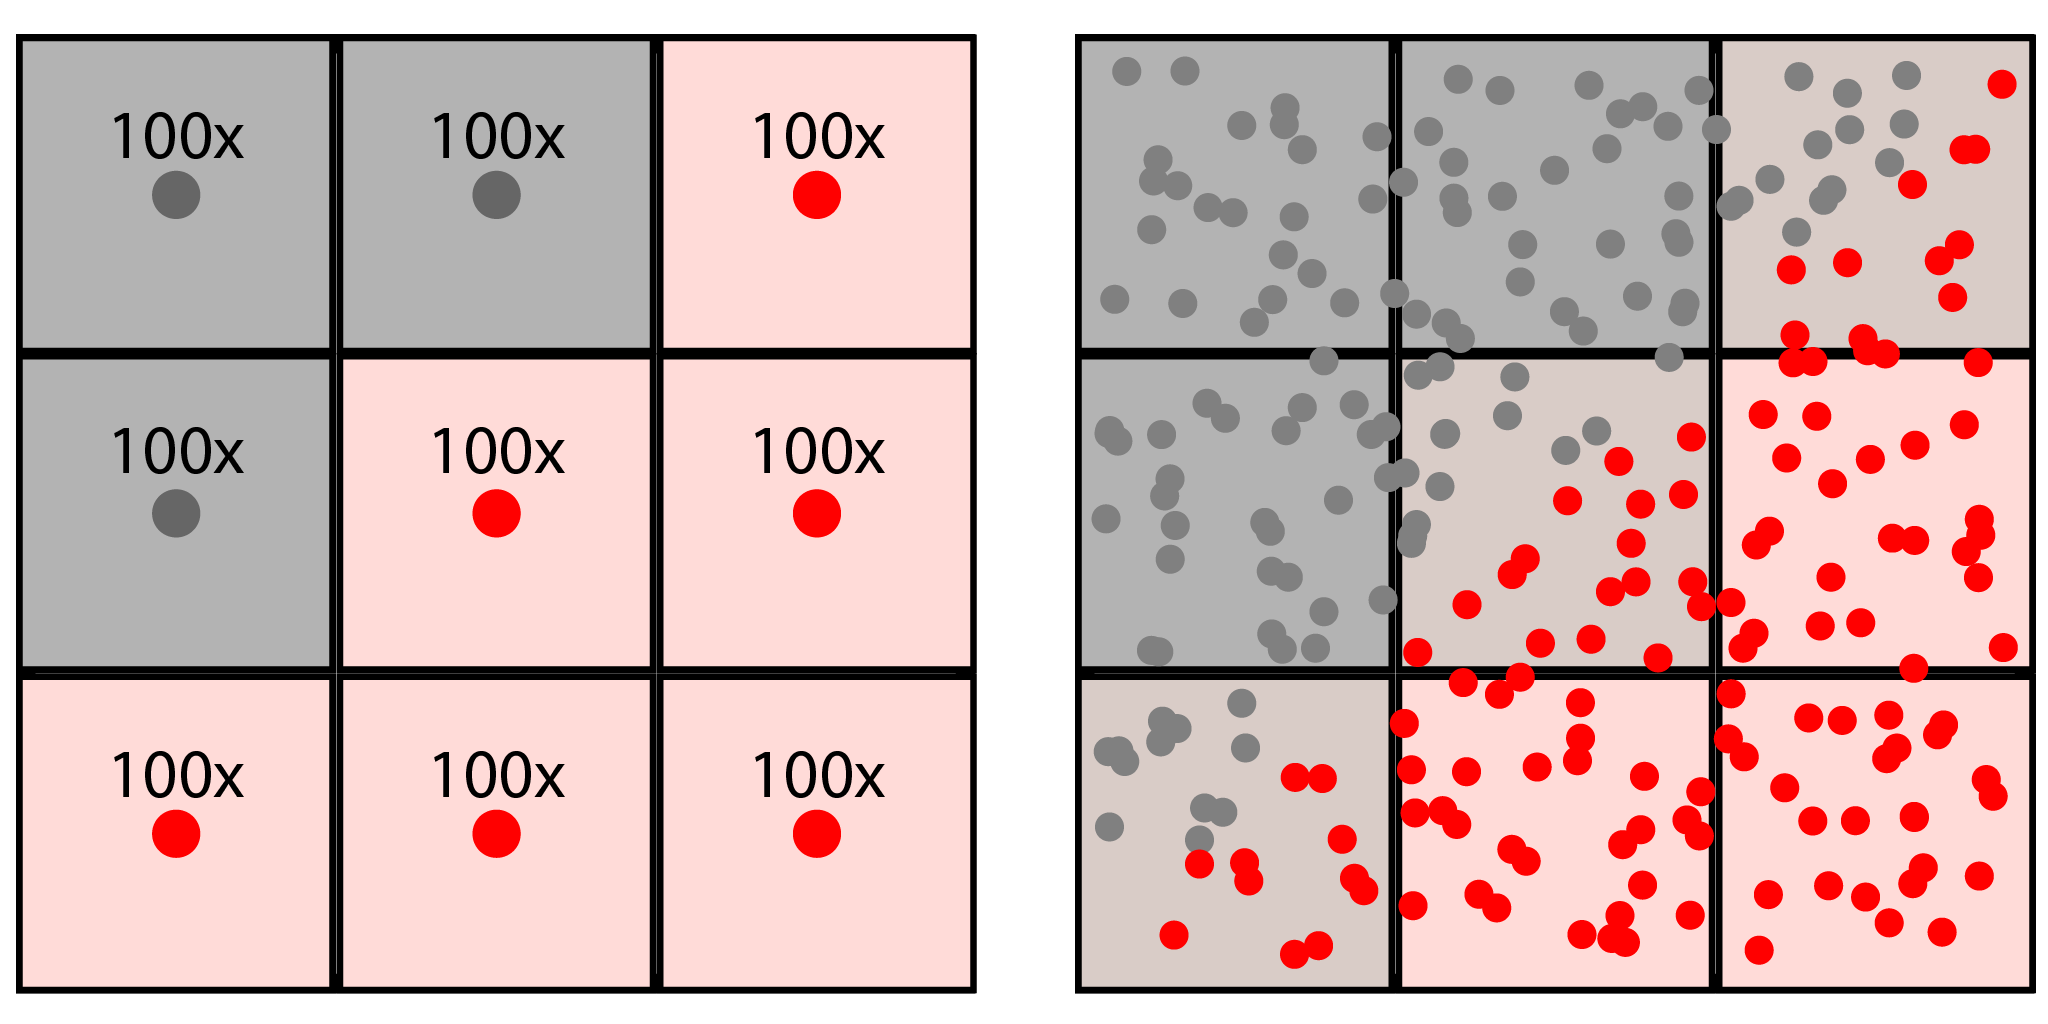
\includegraphics[width=0.9\textwidth]{img/efects AA.png}
\end{frame}


\begin{frame}{Efekty kamery}
Věci které máme témeř zdarma
\begin{itemize}
  \item Anti-aliasing: více paprsků/pixel
  \item \textbf{Depth of field: simulace clony}
  \item Motion blur: čas jako další rozměr
\end{itemize}
\vfill
\centering 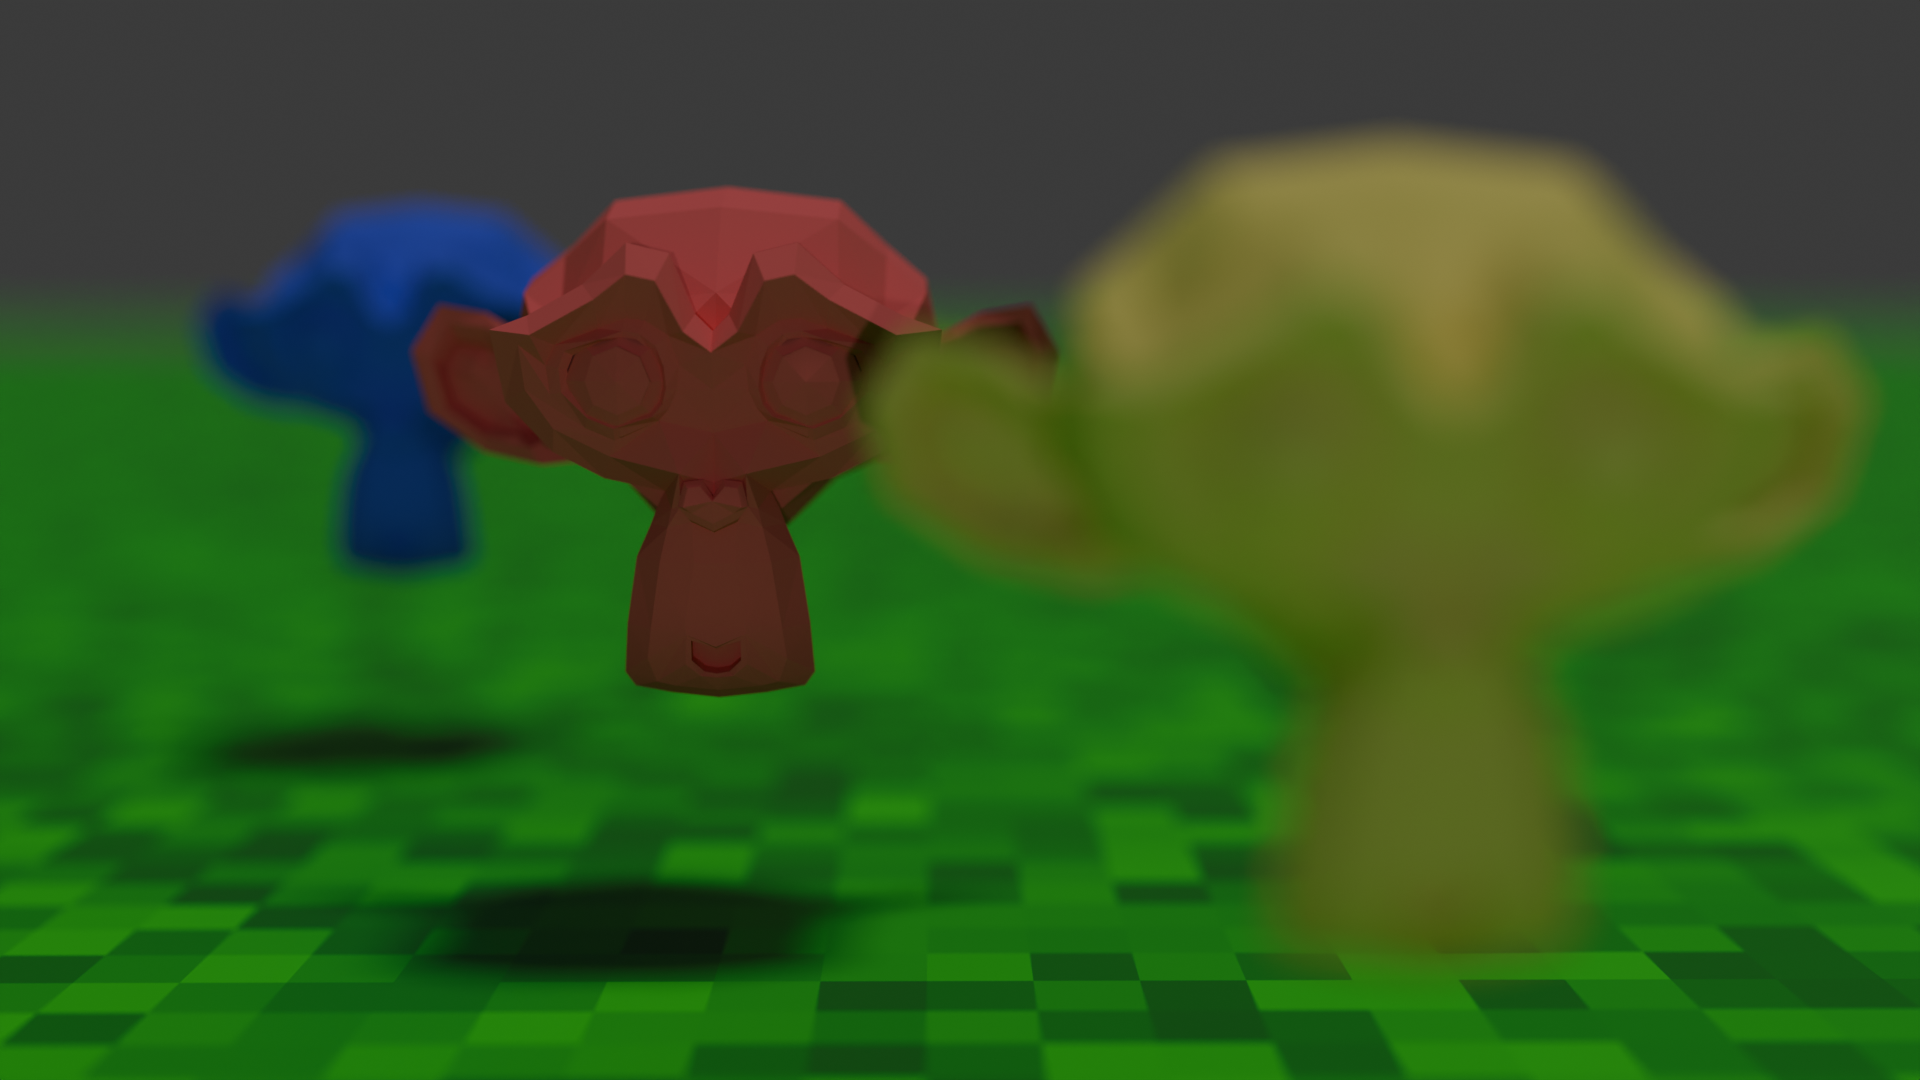
\includegraphics[width=0.8\textwidth]{img/efects DoF.png}
\end{frame}


\begin{frame}{Efekty kamery}
Věci které máme témeř zdarma
\begin{itemize}
  \item Anti-aliasing: více paprsků/pixel
  \item Depth of field: simulace clony
  \item \textbf{Motion blur: čas jako další rozměr}
\end{itemize}
\vfill
\centering {
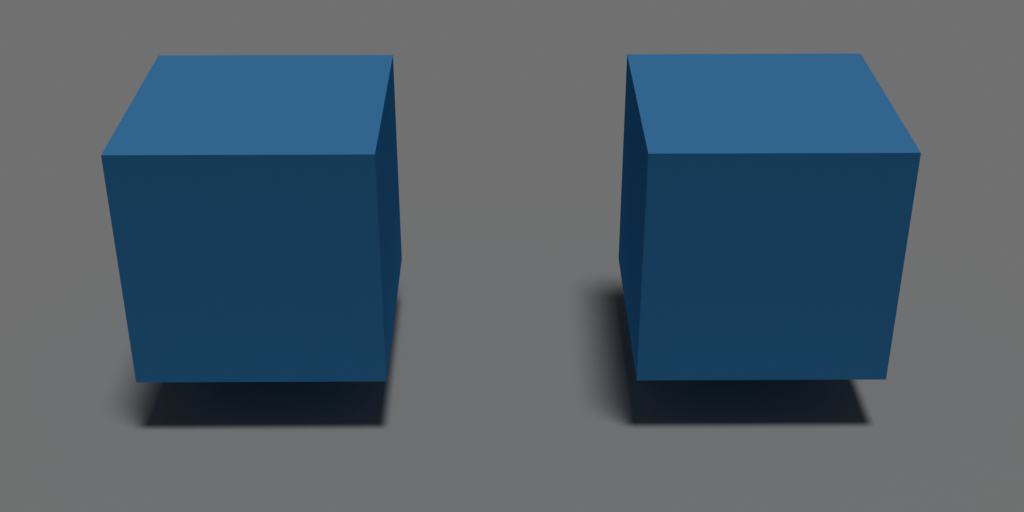
\includegraphics[width=0.47\textwidth]{img/without motion blur.png}
\hfill
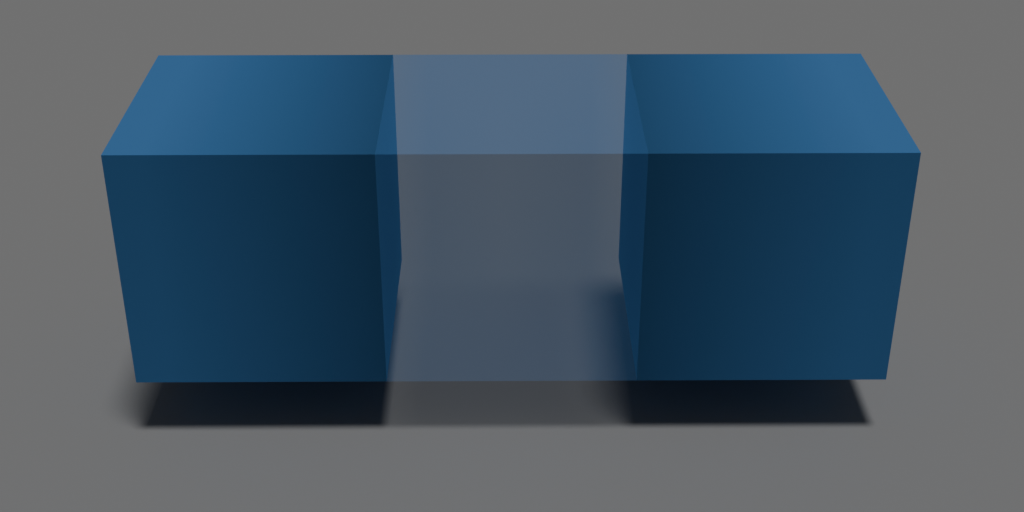
\includegraphics[width=0.47\textwidth]{img/with motion blur.png}
}
\end{frame}


\begin{frame}{Spektrální efekty}
\begin{itemize}
  \item RGB nestačí na všechny jevy
  \item Simulace vlnových délek
  \item Disperze, duhové efekty, fluorescence
\end{itemize}
\centering 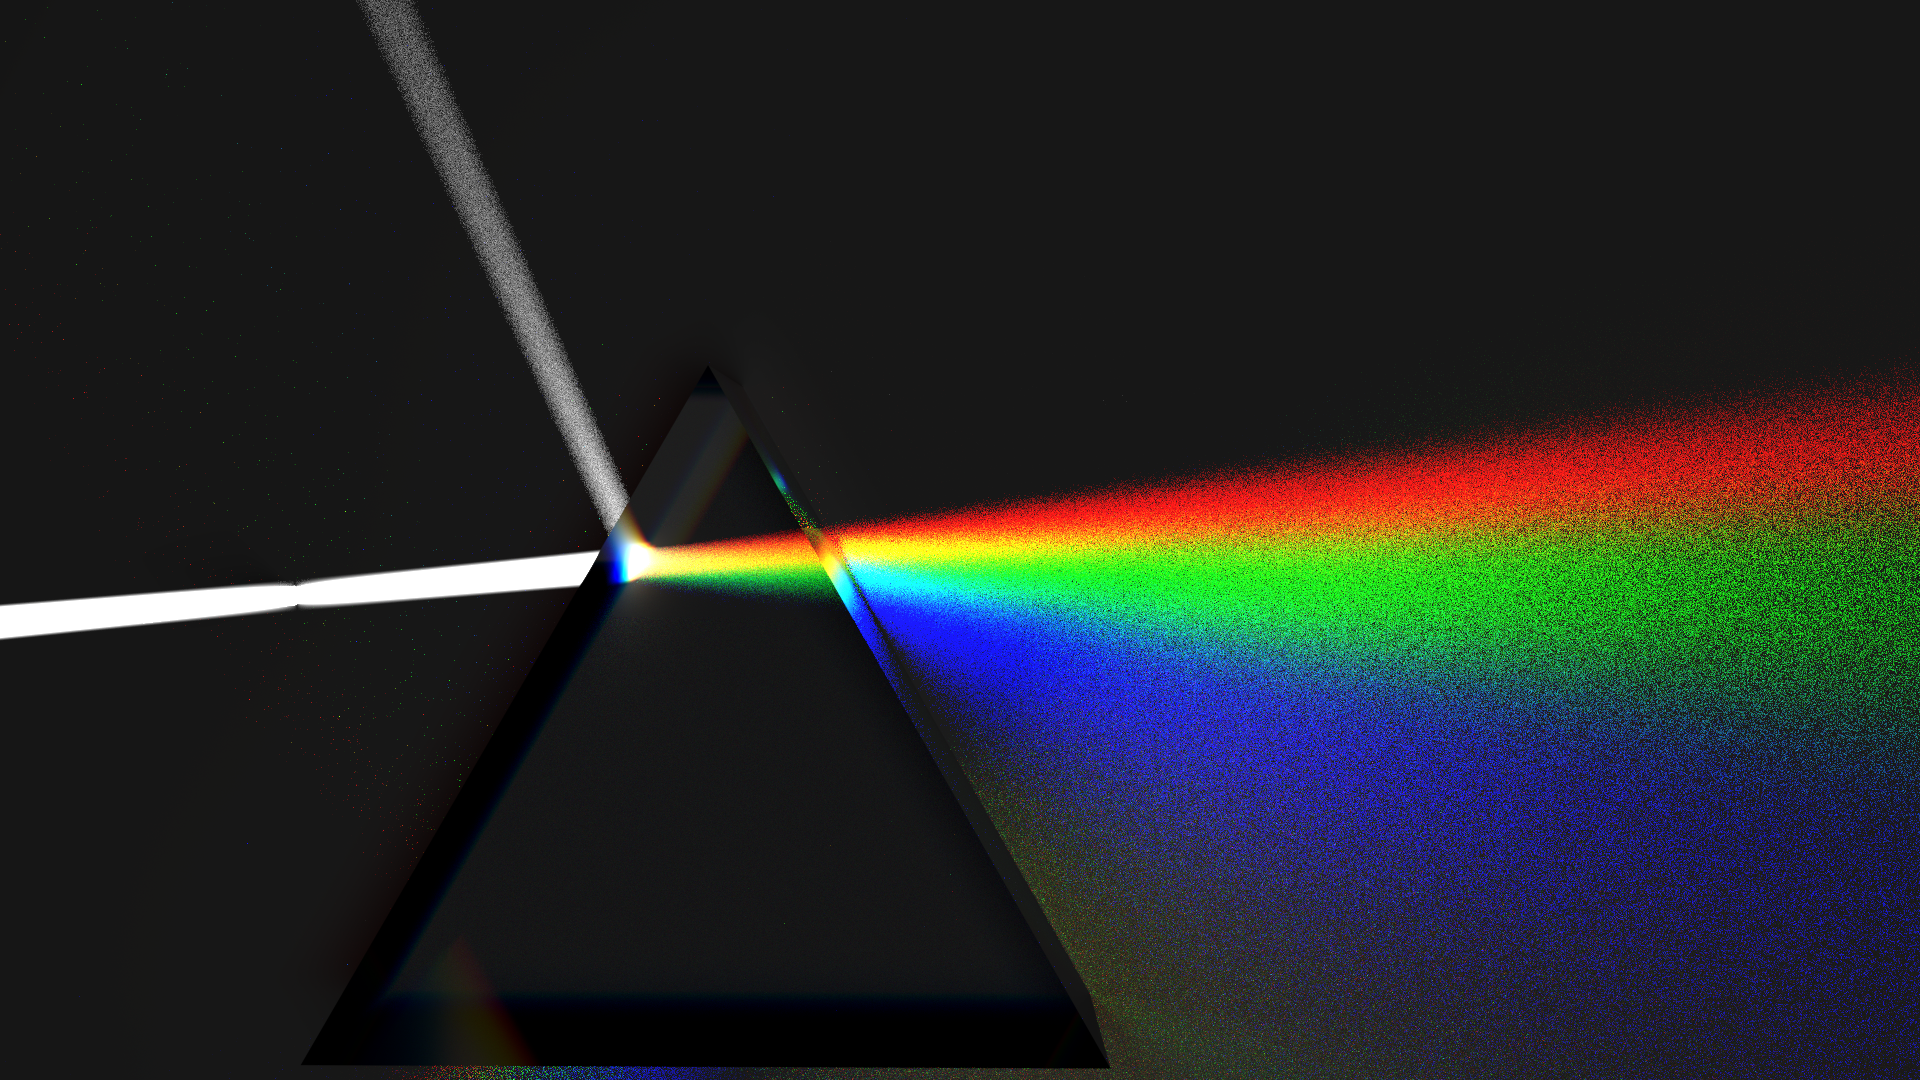
\includegraphics[width=0.8\textwidth]{img/spectrum.png}
\end{frame}


\begin{frame}{Denoising}
\begin{itemize}
  \item Filtrace šumu po renderu
  \item Umožňuje méně paprsků na pixel
\end{itemize}
\vfill
\centering 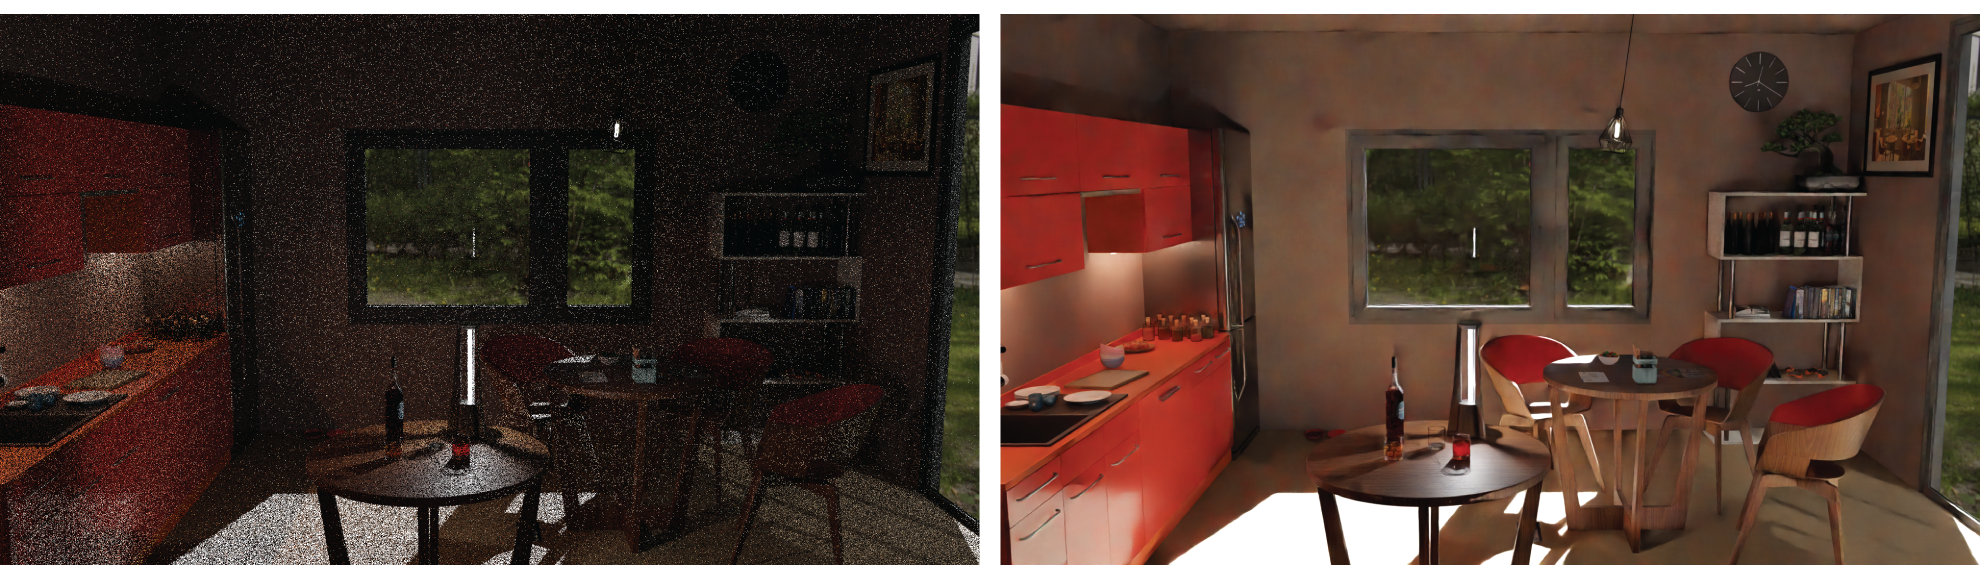
\includegraphics[width=0.95\textwidth]{img/denoise example.png}
\end{frame}


\begin{frame}{Denoising}
\begin{itemize}
  \item Využití algoritmů, AI i pomocných bufferů
\end{itemize}
\vfill
\centering 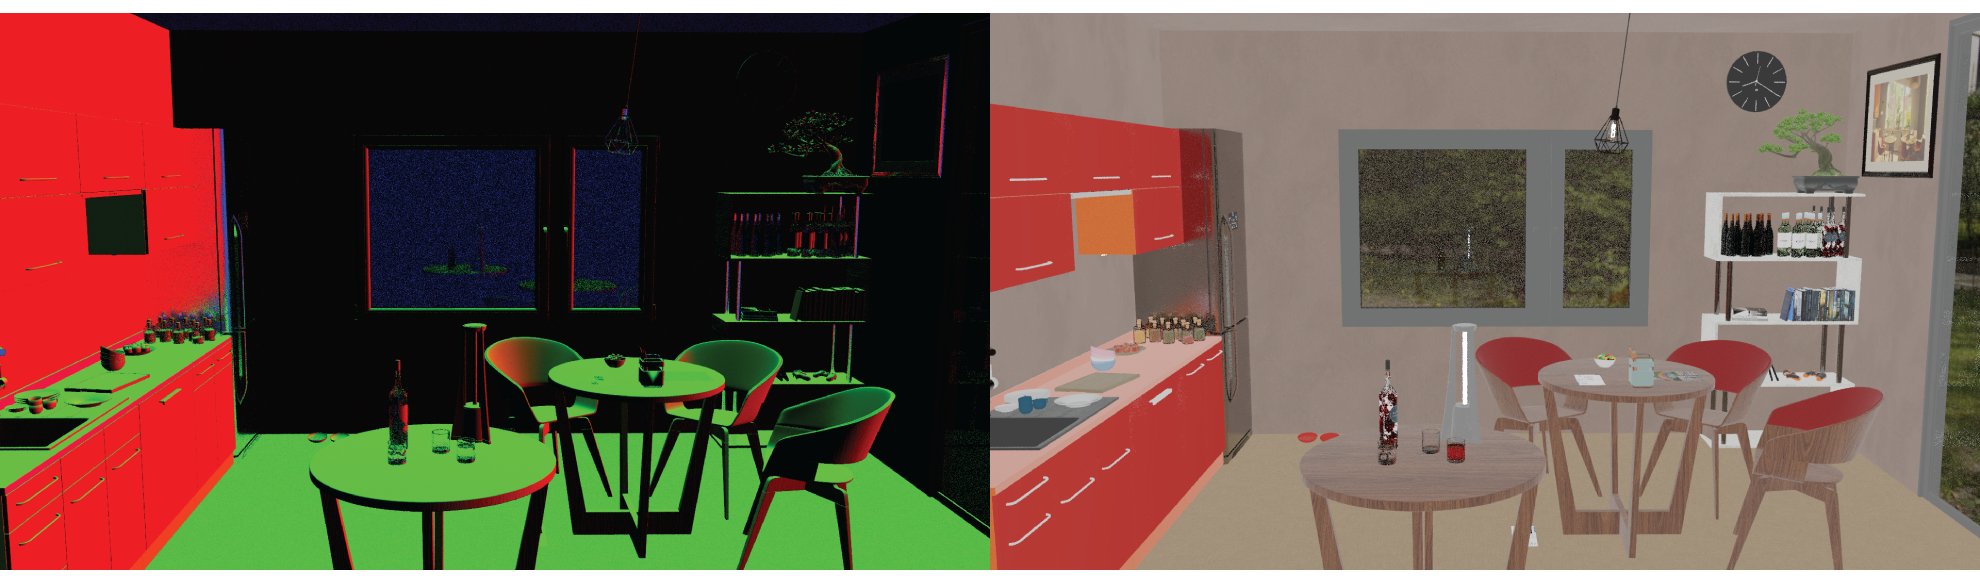
\includegraphics[width=0.95\textwidth]{img/denoise buffers.png}
\end{frame}


\begin{frame}{Denoising}
\begin{itemize}
  \item Porovnání s referenčním obrázkem
\end{itemize}
\vfill
\centering 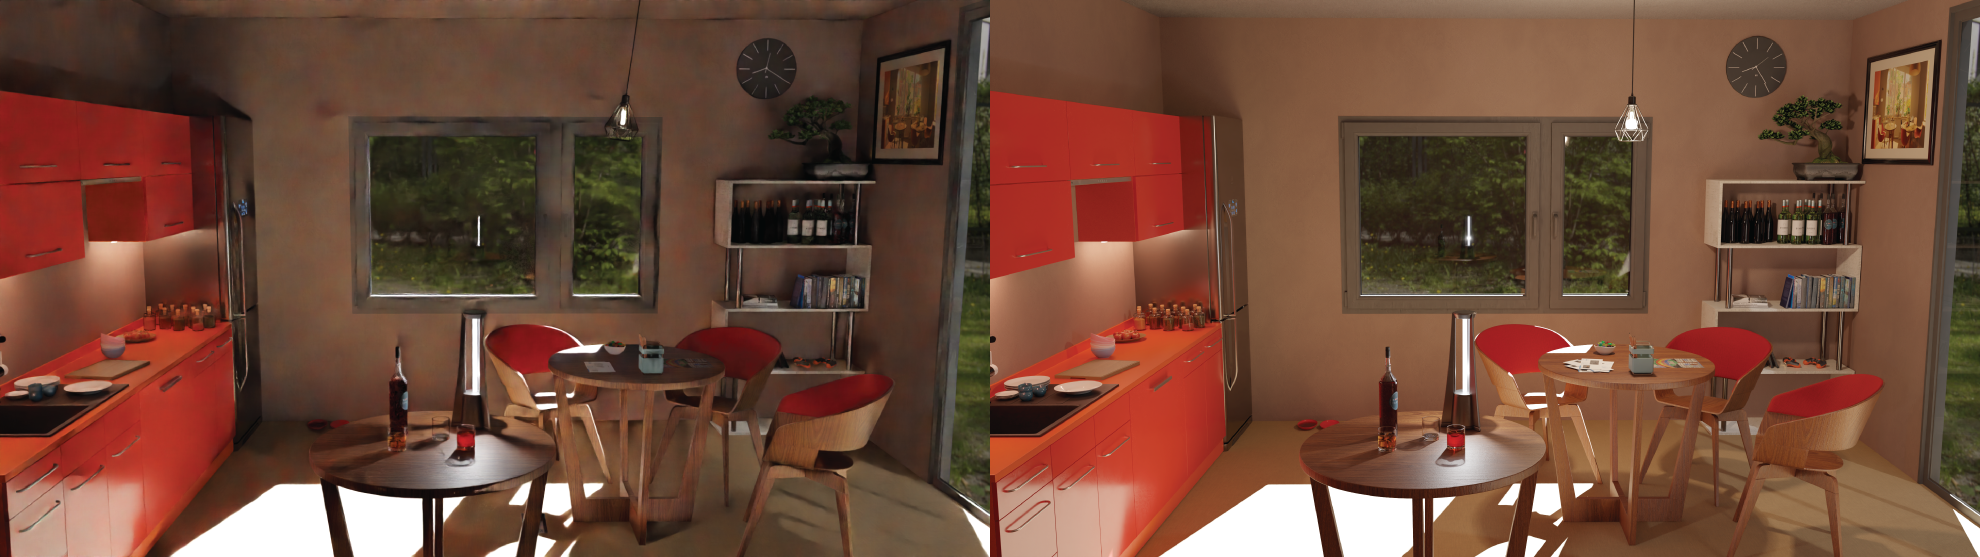
\includegraphics[width=0.95\textwidth]{img/denoise comparison.png}
\\
\centering{1 vzorek na pixel \hskip 60pt 10000 vzorků na pixel}
\end{frame}


\begin{frame}{Hry}
\begin{itemize}
  \item Co kdybychom z 60 vteřin na snímek udělali 60 snímků za vteřinu?
\vfill
\end{itemize}
\centering {
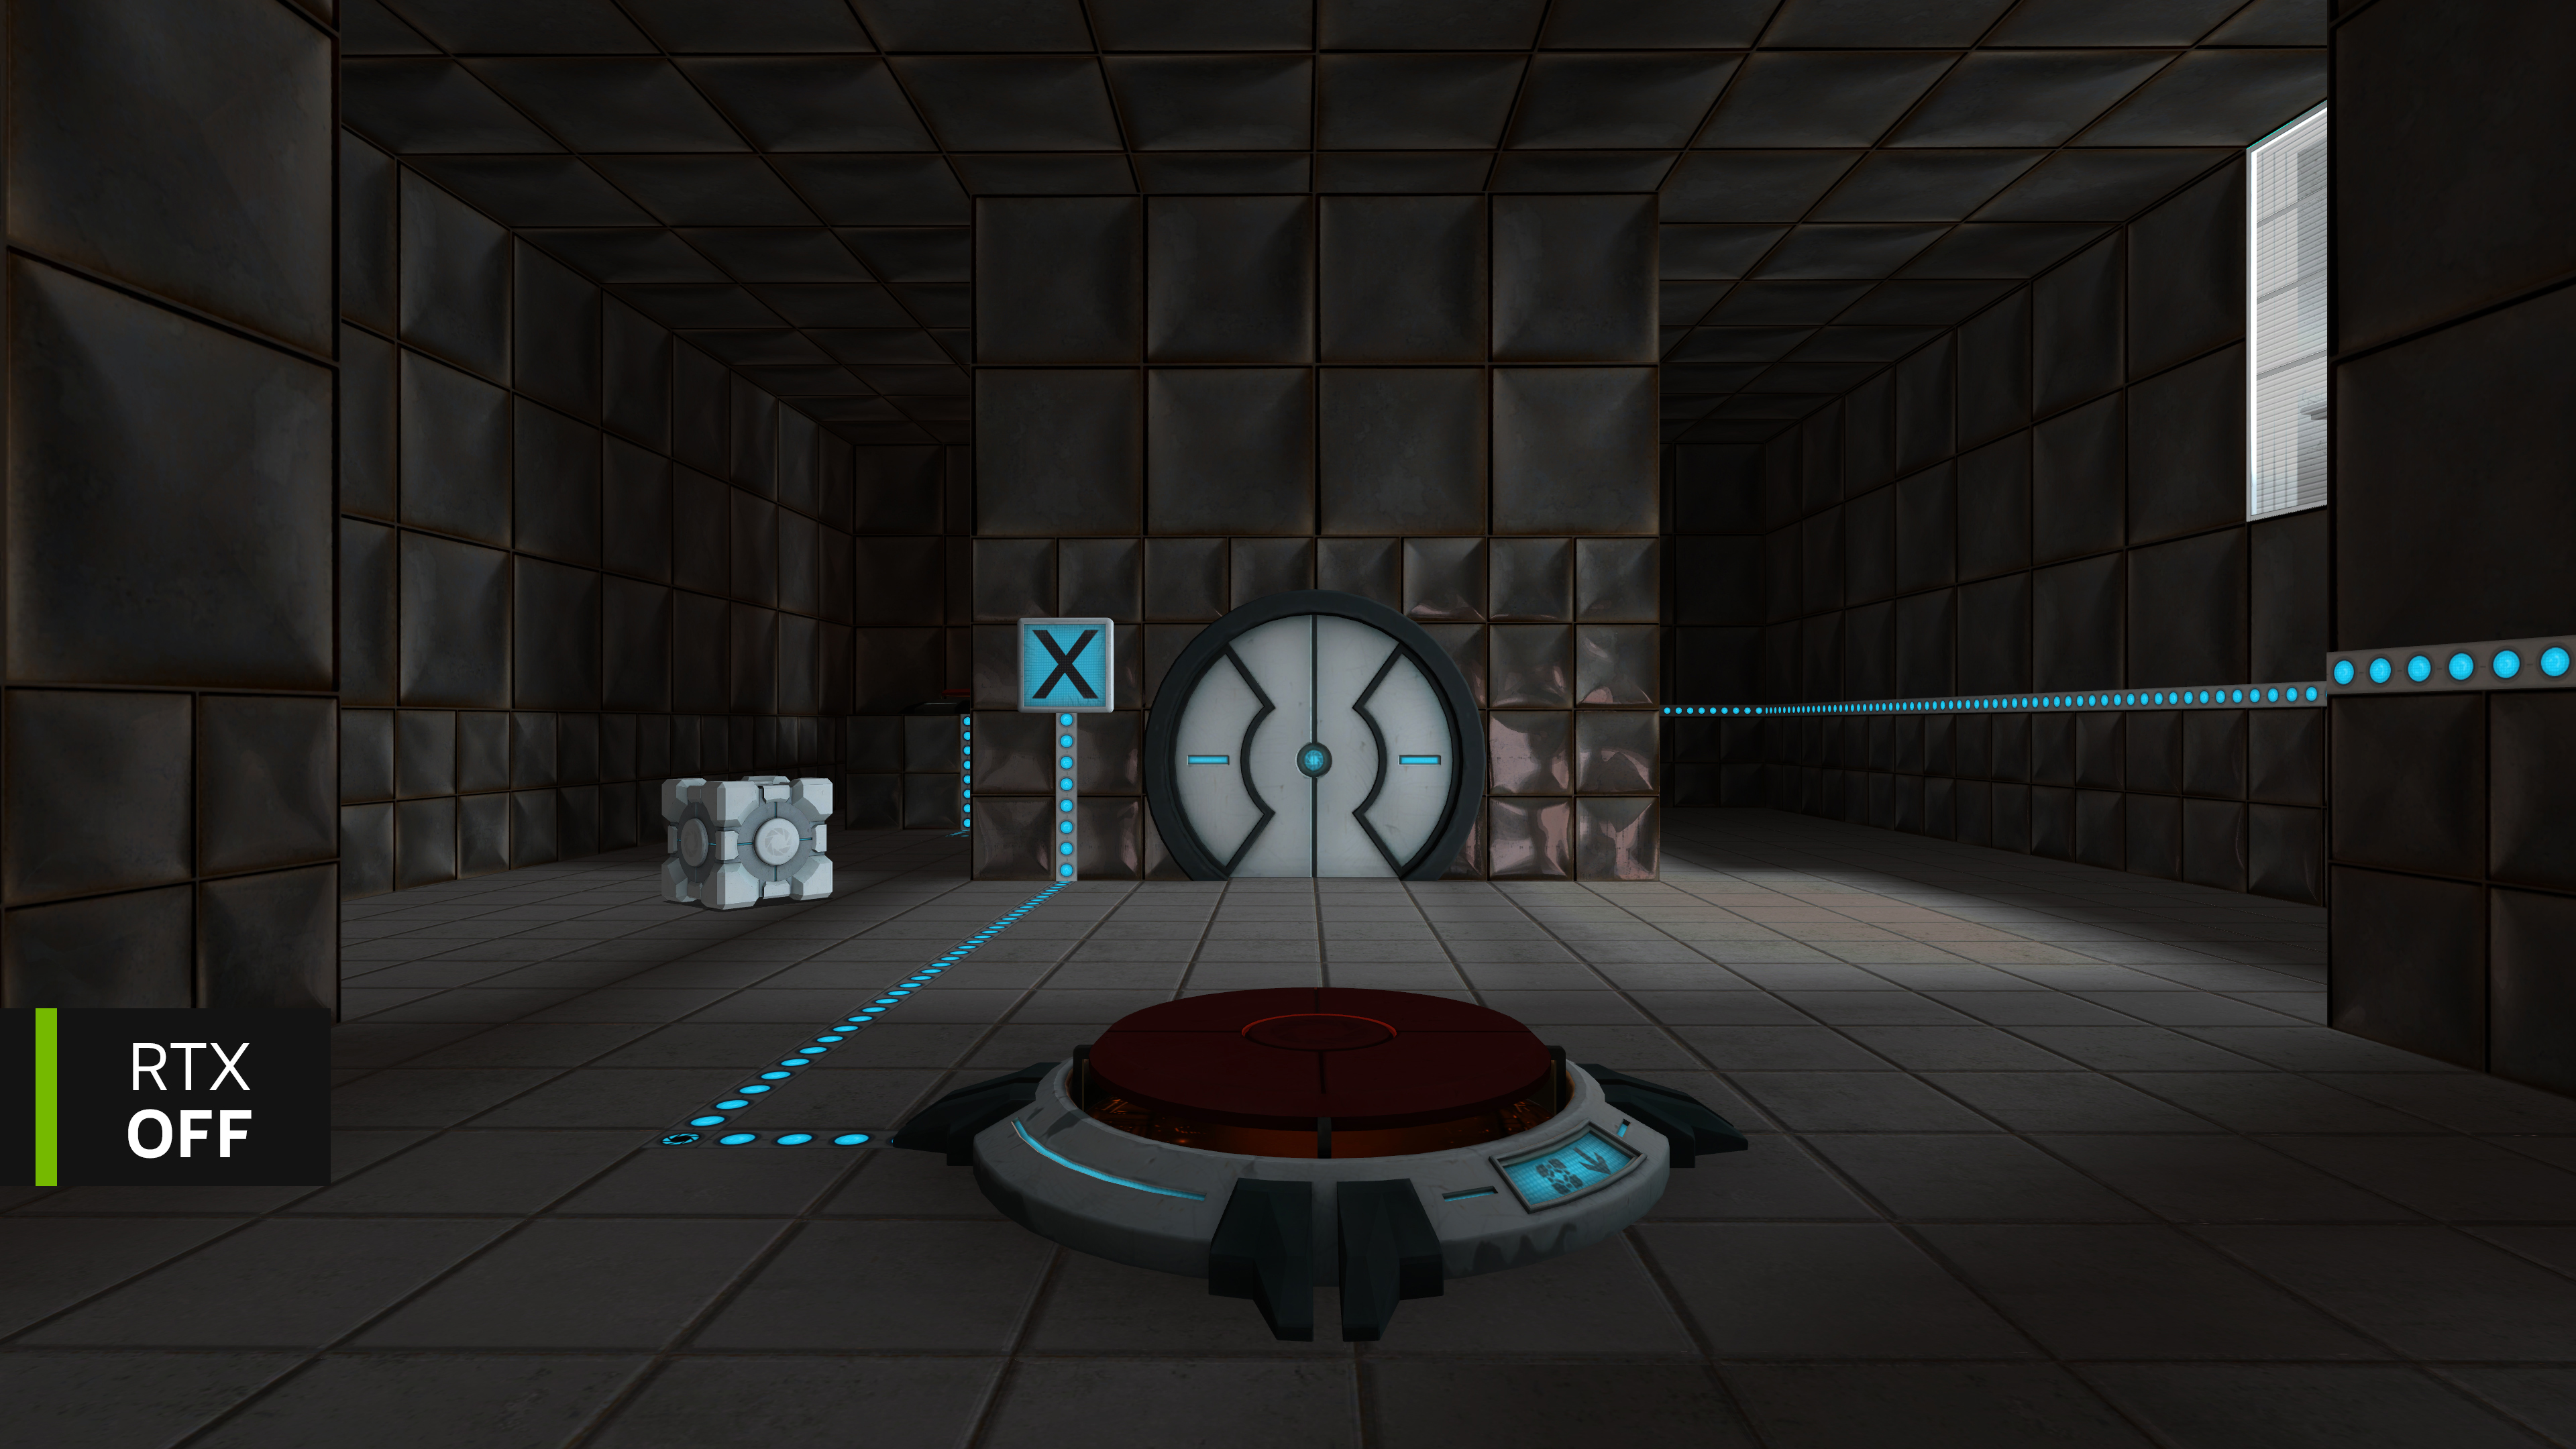
\includegraphics[width=0.48\textwidth]{img/portal.jpg}%
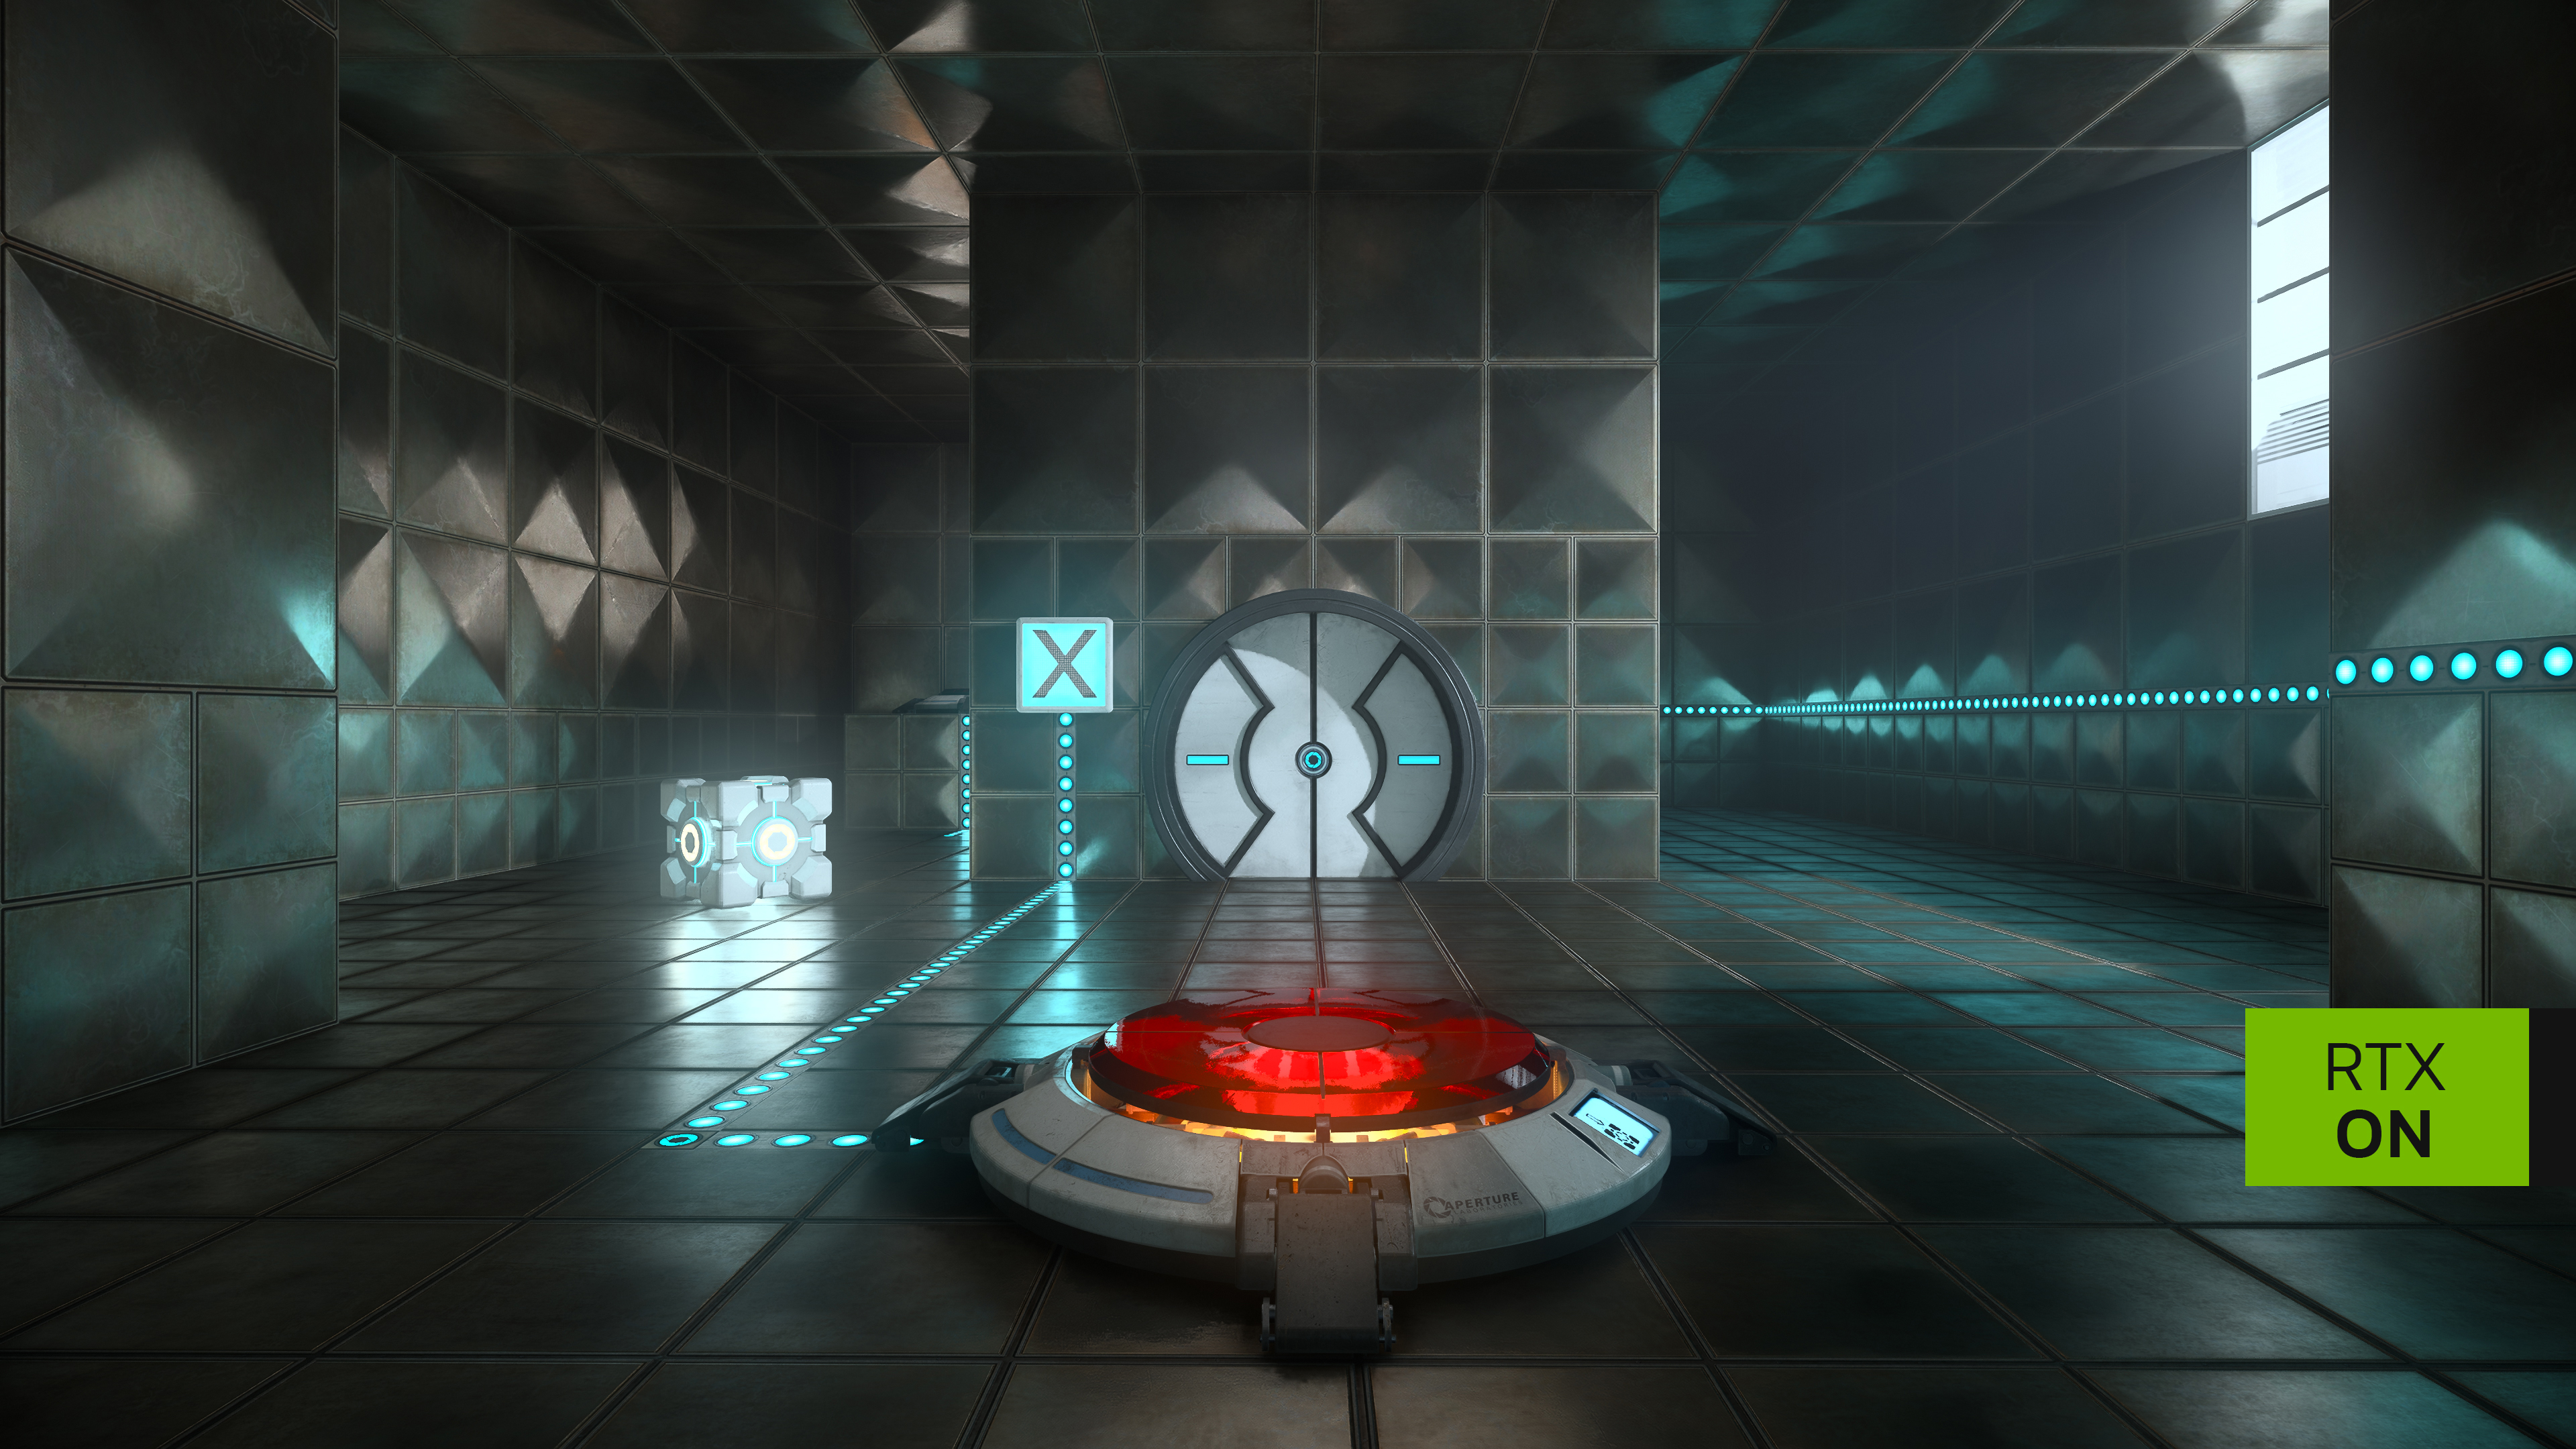
\includegraphics[width=0.48\textwidth]{img/portal rtx.jpg}
\\
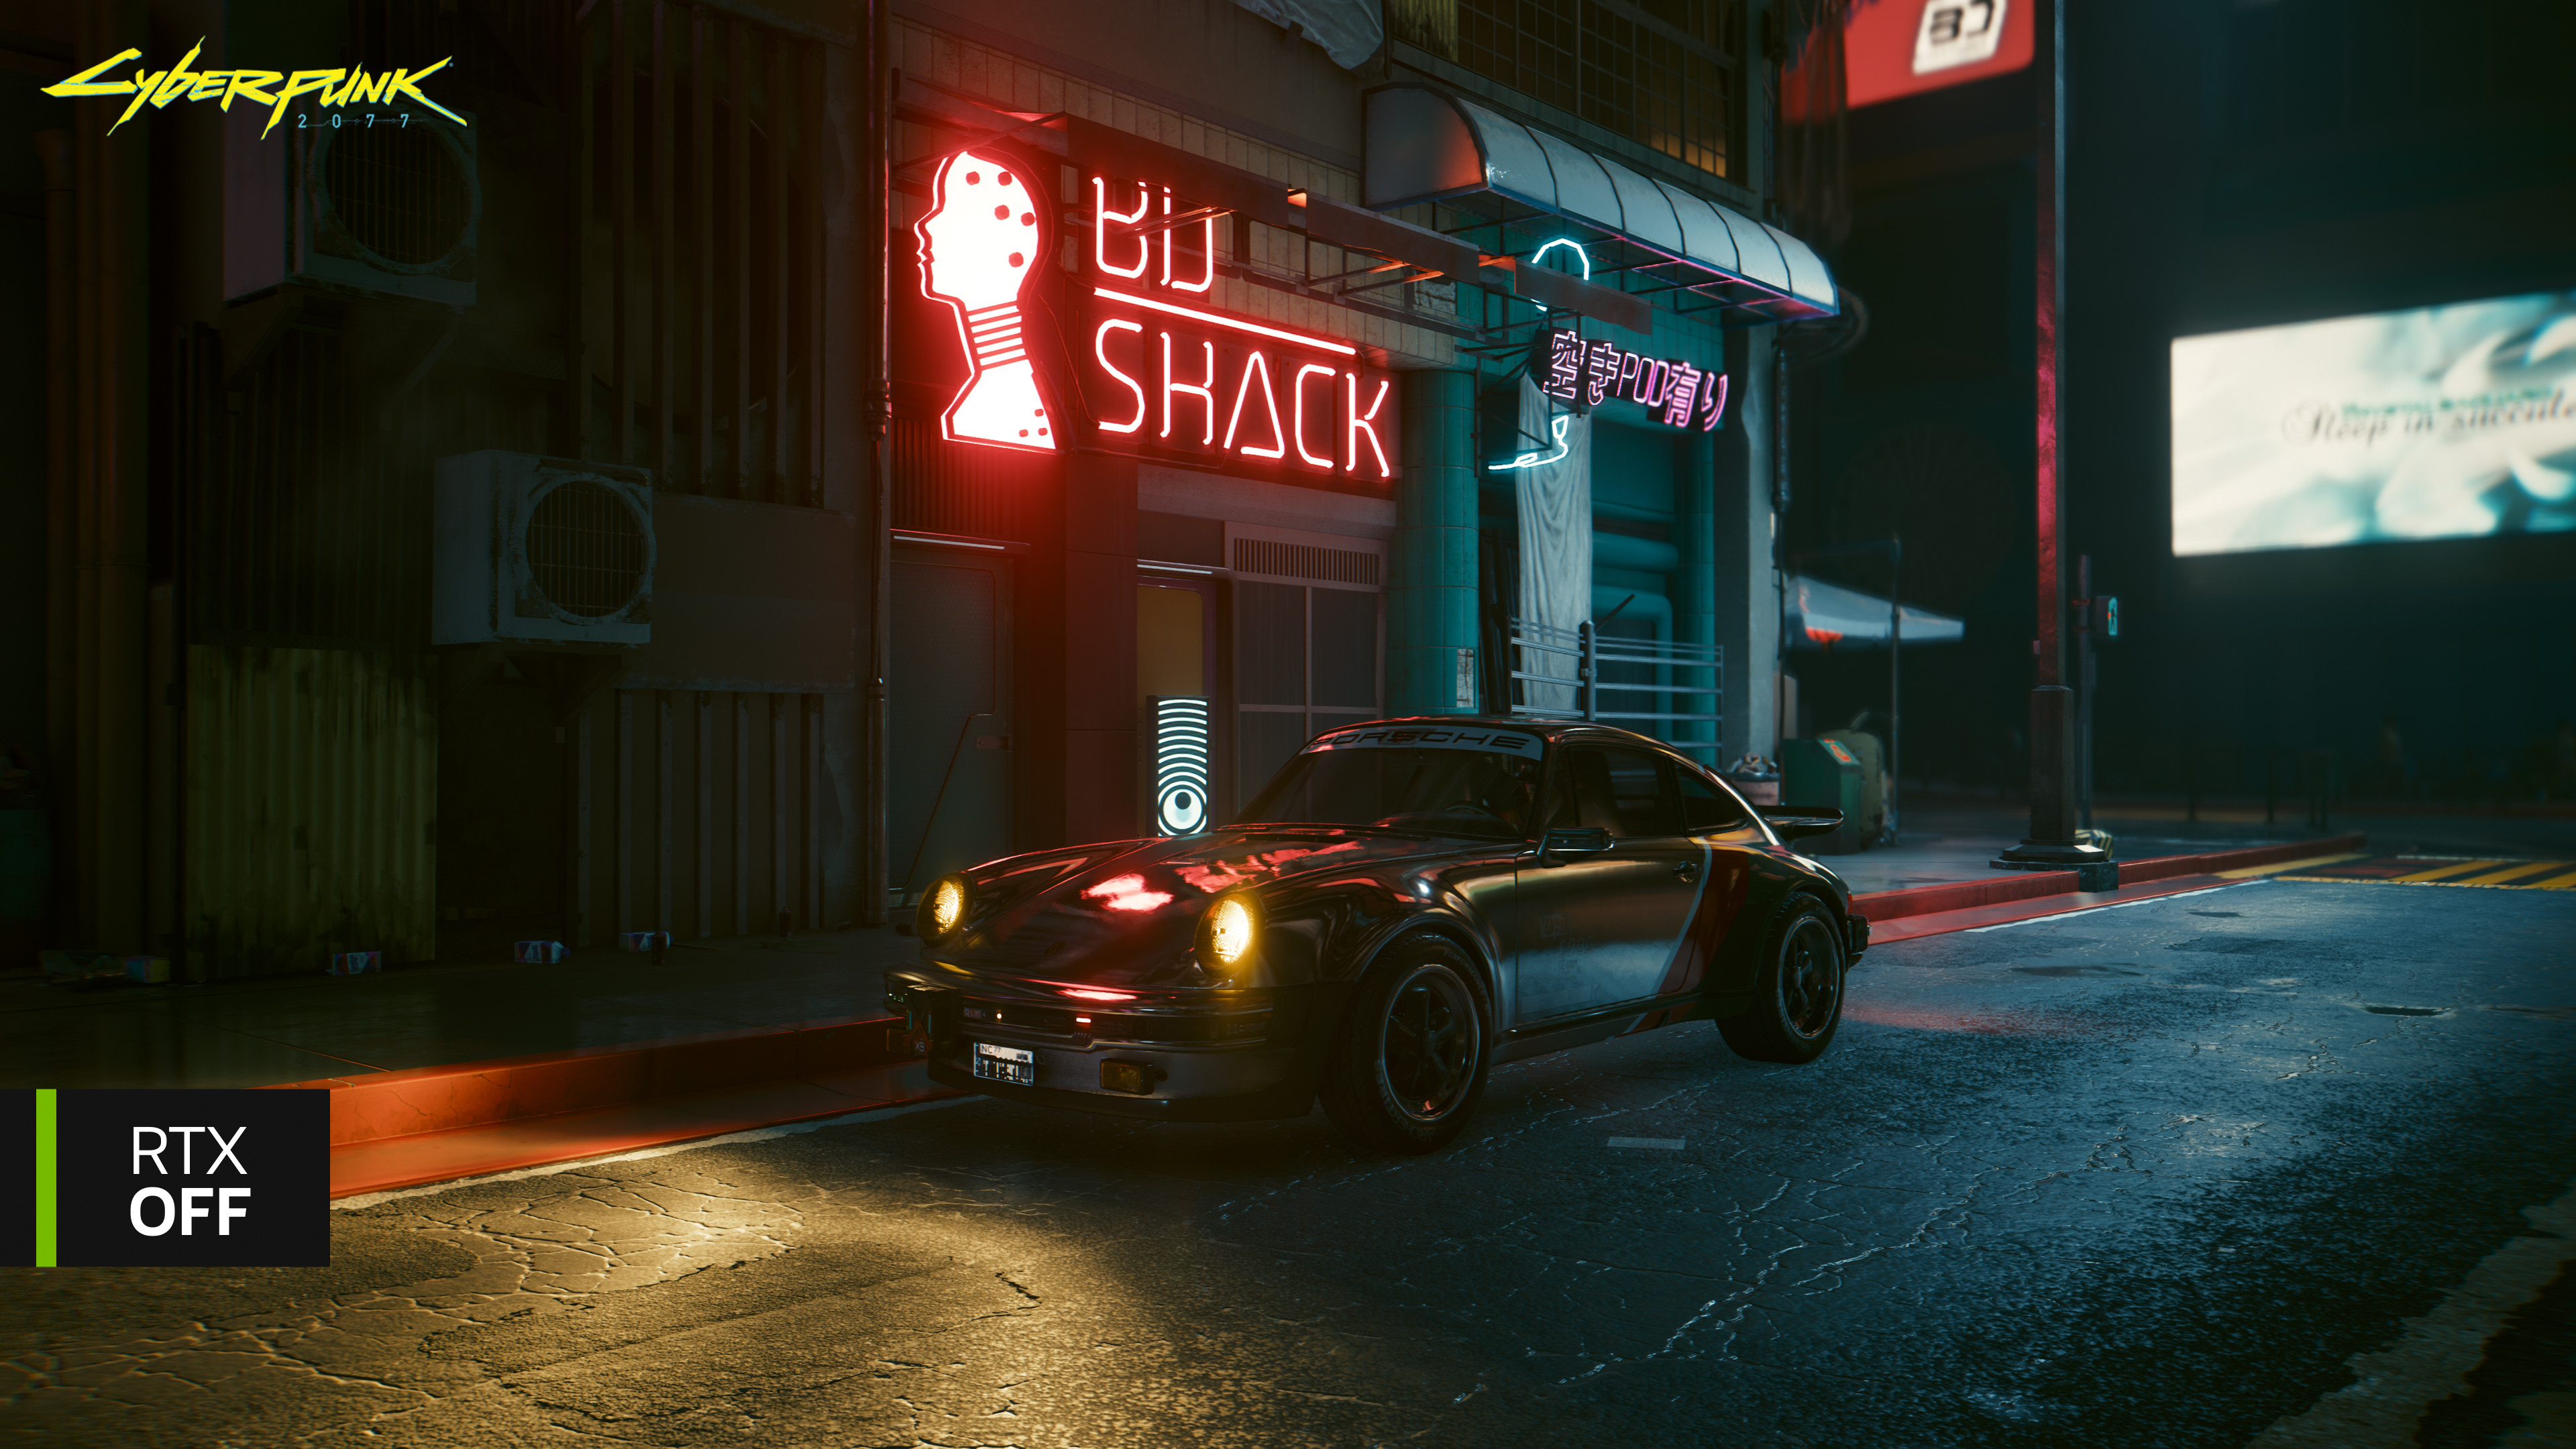
\includegraphics[width=0.48\textwidth]{img/cp2077.jpg}%
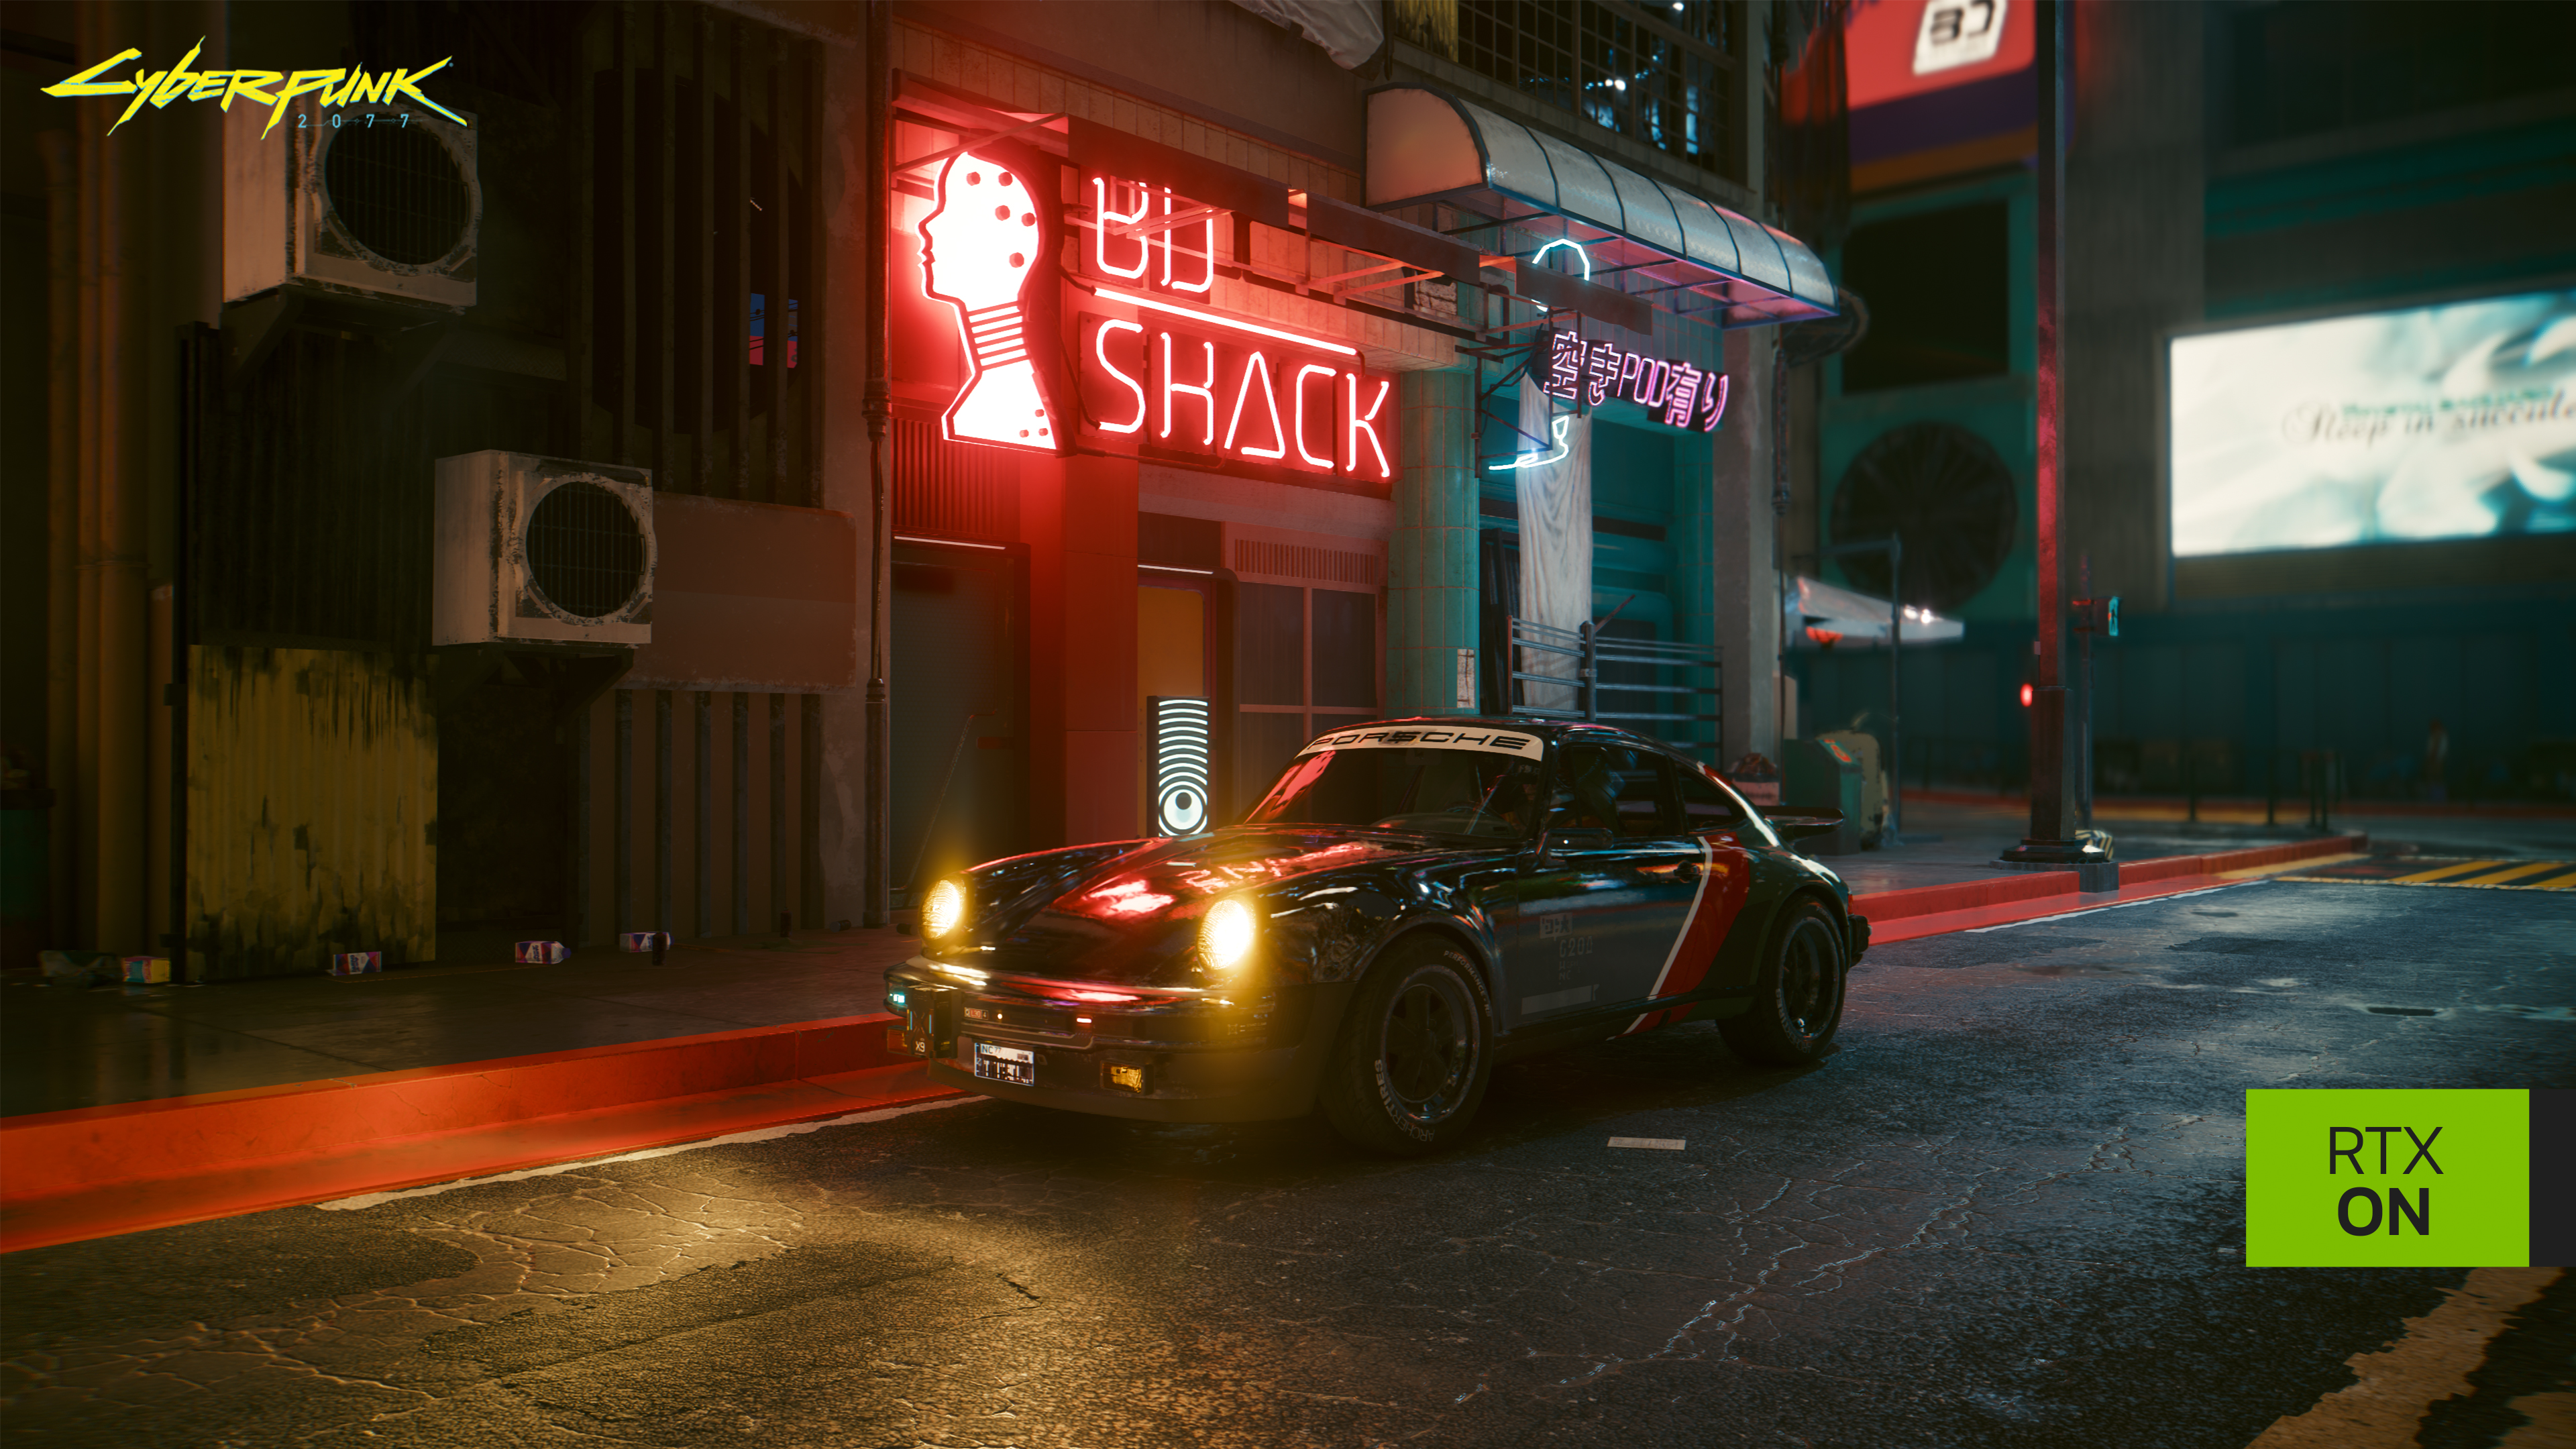
\includegraphics[width=0.48\textwidth]{img/cp2077 rtx.jpg}
\\
{
\fontsize{5.5pt}{5.7pt}\selectfont%
Zdroje: https://www.nvidia.com/en-us/geforce/news/gfecnt/20229/portal-with-rtx-ray-tracing/\\%
https://www.nvidia.com/en-us/geforce/news/cyberpunk-2077-ray-tracing-overdrive-update-launches-april-11/
}
}
\end{frame}


\begin{frame}{Perlička na závěr}
\centering 
\includegraphics[width=1\linewidth]{img/groo.png}
\end{frame}


\end{document}
